\documentclass[12pt]{amsart}
      % \newif\ifpreview
      % \previewfalse

% approx iid
\newcommand\simiid{\stackrel{\mathclap{\normalfont\mbox{\tiny{iid}}}}{\sim}}
\usepackage{natbib}
\usepackage{titlecaps}
\Addlcwords{a about above after again against all am an and any are aren't as at be because been before being below between both but by can't cannot could couldn't did didn't do does doesn't doing don't down during each few for from further had hadn't has hasn't have haven't having he he'd he'll he's her here here's hers herself him himself his how how's i i'd i'll i'm i've if in into is isn't it it's its itself let's me more most mustn't my myself no nor not of off on once only or other ought our ours ourselves out over own same shan't she she'd she'll she's should shouldn't so some such than that that's the their theirs them themselves then there there's these they they'd they'll they're they've this those through to too under until up very was wasn't we we'd we'll we're we've were weren't what what's when when's where where's which while who who's whom why why's with won't would wouldn't you you'd you'll you're you've your yours yourself yourselves}

% Fonts
% at some point figure out bolding ...
\usepackage[default,oldstyle,scale=0.95]{opensans}
%\usepackage[sfdefault,scaled=.85]{FiraSans}
\usepackage[T1]{fontenc}
\usepackage{textcomp}
\usepackage[varqu,varl]{zi4}% inconsolata typewriter
\usepackage{amsmath,amsthm}
\usepackage[cmintegrals]{newtxsf}
\usepackage[T1]{fontenc}
\usepackage{ae}

% easy commands for number propers
\newcommand{\first}{1$^{\text{st}}$}
\newcommand{\second}{2$^{\text{nd}}$}
\newcommand{\third}{3$^{\text{rd}}$}
\newcommand{\nth}[1]{${#1}^{\text{th}}$}

% Generate some fake text
\usepackage{blindtext}

% % add watermark
% \usepackage{draftwatermark}
% \SetWatermarkText{Submission Copy}
% \SetWatermarkScale{.5}
% \SetWatermarkColor[gray]{0.9}

% layout control
\usepackage{geometry}
\geometry{verbose,tmargin=1in,bmargin=1.25in,lmargin=1in,rmargin=1in}
\usepackage{parallel}
\usepackage{parcolumns}
\usepackage{fancyhdr}
\usepackage[export]{adjustbox}
\usepackage{etoolbox}

% math typesetting
\usepackage{array}
\usepackage{amsmath}
\usepackage{amssymb}
\usepackage{amsthm}
\usepackage{amsfonts}
\usepackage{relsize}
\usepackage{mathtools}
\usepackage{bm}
%\usepackage[%decimalsymbol=.,digitsep=fullstop]{siunitx}

% restricts float objects to be inserted before end of section
% creates float barriers
\usepackage[section]{placeins}

% tables
\usepackage{tabularx}
\usepackage{booktabs}
\usepackage{multicol}
\usepackage{multirow}
\usepackage{longtable}

% to adapt caption style
\usepackage[font={small},labelfont=bf]{caption}

% footnotes at bottom
%\usepackage[bottom]{footmisc}

% to change enumeration symbols begin{enumerate}[(a)]
\usepackage{enumerate}
\usepackage{paralist}

% to colorize links in document. See color specification below
\usepackage[pdftex,hyperref,x11names]{xcolor}

% for multiple references and insertion of the word "figure" or "table"
% \usepackage{cleveref}

% load the hyper-references package and set document info
\usepackage[pdftex]{hyperref}

% graphics stuff
\usepackage{subfigure}
\usepackage{graphicx}
\usepackage[space]{grffile} % allows us to specify directories that have spaces
\usepackage{placeins} % prevents floats from moving past a \FloatBarrier
\usepackage{tikz}

% sideway figures
\usepackage{rotating}
\usepackage{lscape}

%\usepackage[figuresright]{rotating}
% \newenvironment{amssidewaysfigure}  {\begin{sidewaysfigure}\vspace*{.8\textwidth}\begin{minipage}{\textheight}\centering}
%   {\end{minipage}\end{sidewaysfigure}}

% Spacing
\usepackage[doublespacing]{setspace}

% outside code
\usepackage{listings}
\usepackage{enumitem}

% define clickable links and their colors
\hypersetup{%
	unicode=false,          % non-Latin characters in Acrobat's bookmarks
	pdftoolbar=true,        % show Acrobat's toolbar?
	pdfmenubar=true,        % show Acrobat's menu?
	pdffitwindow=false,     % window fit to page when opened
	pdfstartview={FitH},    % fits the width of the page to the window
	pdfnewwindow=true,%
	%pagebackref=false,%
	pdfauthor={Shahryar Minhas, et alia.},%
	pdftitle={Taking Dyads Seriously},%
	colorlinks,%
	citecolor=black,%
	filecolor=black,%
	linkcolor=black,%
	urlcolor=RoyalBlue4
}

% -------------------- title -------------------- %

\title{Taking Dyads Seriously}
\vspace{\baselineskip}

% \author[Minhas]{Shahryar Minhas}
% \address{Shahryar Minhas: Department of Political Science}
% \curraddr{Michigan State University}
% \email[Corresponding author]{minhassh@msu.edu}

% \author[Dorff]{Cassy L. Dorff}
% \address{Cassy L. Dorff}
% \curraddr{Department of Political Science, University of New Mexico}
% \email{cdorff@unm.edu}

% \author[Foster]{Margaret Foster}
% \address{Margaret Foster}
% \curraddr{Department of Political Science, Duke University}
% \email{margaret.foster@duke.edu}

% \author[Gallop]{Max Gallop}
% \address{Max Gallop}
% \curraddr{Department of Government and Public Policy, University of Strathclyde}
% \email{max.gallop@strath.ac.uk}

% \author[Liu]{Howard Liu}
% \address{Howard Liu}
% \curraddr{Department of Political Science, Duke University}
% \email{hao.liu@duke.edu}

% \author[Tellez]{Juan Tellez}
% \address{Juan Tellez}
% \curraddr{Department of Political Science, Duke University}
% \email{juan.tellez@duke.edu}

% \author[Ward]{Michael D. Ward}
% \address{Michael D. Ward}
% \curraddr{Department of Political Science, Duke University}
% \email{michael.d.ward@duke.edu}

% \date{\today}

% \thanks{Shahryar Minhas and Michael D. Ward acknowledge support from National Science Foundation (NSF) Award 1259266. Peter Hoff, John Ahlquist, Robert Franzese, Arturas Rozenas, Betsy Sinclair, Jacob Montgomery and Benjamin Appel provided welcome and helpful comments. We also thank Douglas Gibler for kindly providing us with a copy of the data and programs he used in \citet{gibler:2017}. We benefited from presentations of this material at the 2017 Political Methodology Conference, and our home institutions.}

\setlength{\headheight}{15pt}
\setlength{\headsep}{20pt}
\pagestyle{fancyplain}
\fancyhf{}
\lhead{\fancyplain{}{}}
% \chead{\fancyplain{}{Taking Dyads Seriously}}
\chead{\fancyplain{}{}}
% \rhead{\fancyplain{}{\today}}
\rhead{\fancyplain{}{}}
\rfoot{\fancyplain{}{\thepage}}

% references to graphics
\makeatletter
% \def\input@path{{/Users/janus829/Dropbox/toDo_notes/nsfSumm/Graphics/}, {/Users/s7m/Dropbox/toDo_notes/nsfSumm/Graphics/}}
% \graphicspath{{/Users/janus829/Dropbox/toDo_notes/nsfSumm/Graphics/}, {/Users/s7m/Dropbox/toDo_notes/nsfSumm/Graphics/}}

% easy command for boldface math symbols
\newcommand{\mbs}[1]{\boldsymbol{#1}}

% command for R package font
\newcommand{\pkg}[1]{{\fontseries{b}\selectfont #1}}

% Add some colors
\definecolor{red1}{RGB}{253,219,199}
\definecolor{red2}{RGB}{244,165,130}
\definecolor{red3}{RGB}{178,24,43}

\definecolor{green1}{RGB}{229,245,224}
\definecolor{green2}{RGB}{161,217,155}
\definecolor{green3}{RGB}{49,163,84}

\definecolor{blue0}{RGB}{255,247,251}
\definecolor{blue1}{RGB}{222,235,247}
\definecolor{blue2}{RGB}{158,202,225}
\definecolor{blue3}{RGB}{49,130,189}
\definecolor{blue4}{RGB}{4,90,141}

\definecolor{purple1}{RGB}{191,211,230}
\definecolor{purple2}{RGB}{140,150,198}
\definecolor{purple3}{RGB}{140,107,177}

\definecolor{brown1}{RGB}{246,232,195}
\definecolor{brown2}{RGB}{223,194,125}
\definecolor{brown3}{RGB}{191,129,45}

% square bracket matrices
\let\bbordermatrix\bordermatrix
\patchcmd{\bbordermatrix}{8.75}{4.75}{}{}
\patchcmd{\bbordermatrix}{\left(}{\left[}{}{}
\patchcmd{\bbordermatrix}{\right)}{\right]}{}{}


\begin{document}
% \ifpreview {
%    \definecolor{personal}{rgb}{1.0, 1.0, 0.0}
%    \pagecolor{personal}
%    }
% \fi


\small{\singlespacing{
\begin{abstract}
	International relations scholarship concerns dyads, yet standard modeling approaches fail to adequately capture the data generating process behind dyadic events and processes. As a result, they suffer from biased coefficients and poorly calibrated standard errors. We show how a regression-based approach, the Additive and Multiplicative Effects (AME) model, can be used to account for the inherent dependencies in dyadic data and glean substantive sights in the interrelations between actors. First, we conduct a simulation to highlight how the model captures dependencies and show that accounting for these processes improves our ability to conduct inference on dyadic data. Second, we compare the AME model to approaches used in three prominent studies from recent international relations scholarship. For each study, we find that compared to AME, the modeling approach used performs notably worse at capturing the data generating process. Further, conventional methods misstate the effect of key variables and the uncertainty in these effects. Finally, AME outperforms standard approaches in terms of out-of-sample fit. In sum, our work shows the consequences of failing to take the dependencies inherent to dyadic data seriously. Most importantly, by better modeling the data generating process underlying political phenomena, the AME framework improves scholars' ability to conduct inferential analyses on dyadic data.
\end{abstract}
}}


\maketitle

\begin{center}
	\textbf{Word count}: 9,177
\end{center}

\thispagestyle{empty}
\newpage\setcounter{page}{1}

\section{\textbf{Introduction}}

\citet{aronow:etal:2015} estimate that during the period 2010 to 2015, over sixty articles were published in the \textit{American Political Science Review}, \textit{American Journal of Political Science}, and \textit{International Organization} using dyadic data.\footnote{In 2017, \textit{International Studies Quarterly} published a special issue on Dyadic Research Designs along with an online symposium to discuss the papers.} Most of these studies use a generalized linear model (GLM) to test hypothesized relationships.  However, this approach to studying dyadic data increases the chance of faulty inferences by assuming data are conditionally independent and identically distributed (iid). Most standard approaches assume that the problems raised by having non-iid relational data can be addressed by recalculating the standard errors of estimated parameters to reflect the potential clustering of cases. In practice, such strategies rarely work because they do not directly address the fundamental data generating process. This is important to consider since the inferential problems caused by non-iid  observations affect more than just diagonals of the variance co-variance matrix. \citep{beck:2012,franzese:hayes:2007,king:roberts:2014}.

In this article, we present the Additive and Multiplicative Effects (AME) model, a Bayesian approach for directly modeling relational data to better reflect the interdependencies underlying the data generating process of dyadic data structures \citep{hoff:2008,minhas:etal:2016:arxiv}. We focus on three types of interdependencies that can complicate dyadic analyses. First, dependencies may arise within a set of dyads if a particular actor is more likely to send or receive actions such as conflict.\footnote{In the case of undirected data where there is no clear sender or receiver, it is still essential to take into account the variance in how active actors are in the system.} Additionally, if the event of interest has a clear sender and receiver, we are likely to observe dependencies within a dyad; for example, if a rebel group initiates a conflict against a government, the government will likely reciprocate that behavior. We capture these effects, often referred to as first- and second-order dependencies, respectively, within the additive effects portion of the model. Third order dependencies capture relationships of transitivity, balance, and clusterability between different dyads--for example, we can only understand why Poland was involved in a dyadic conflict with Iraq in 2003 if we understand that the United States invaded Iraq in 2003 and that Poland often participates in US-led coalitions. The multiplicative effects capture these sorts of dependencies, especially those that result because the specified model has not accounted for a latent set of shared attributes that affect actors' probability of interacting with one another.  

We begin with a discussion of these dependencies and an introduction to the AME model. Next, we conduct a simulation study to show how the AME approach can recover unbiased and well-calibrated regression coefficients in the context of dyadic data. Last, to highlight the utility of this approach, we apply the AME model to three recent studies in the international relations (IR) literature. The comparison reveals that in accounting for observational dependence, AME produces more precise estimates and better-calibrated confidence intervals for key variables in the literature. Consequently, AME produces results that, at times, differ from those found in the original study as well as from the broader literature. Moreover, we demonstrate the latent factor approach offers substantive insights that are often occluded by ignoring the interdependencies found in the relational data of IR studies. Finally, we show that for each replication our network-based approach provides substantively more accurate out-of-sample predictions than the models used in the original studies. 

The framework that we present advances statistical analysis of dyadic data by accounting for observational dependence while allowing scholars to test the substantive effect of variables of interest. Thus, the AME approach can be used by scholars in the field to continue to generate substantive insights, while accounting for the data generating process behind political events of interest. Most importantly, the AME approach concentrates on the relational aspect of the field of international relations through a statistical framework that is familiar to most scholars.
\section{\textbf{Dependencies in Dyadic Data}}

Scholars working with dyadic data typically begin by stacking observations associated with each dyad on top of one another. This makes sense if each observation is independent of the others. For example, a conflict initiated from the United States against Japan is assumed to be independent of any conflictual action that Japan may send to the United States. Additionally, every action sent by Japan to others in the system is considered independent even though each of those interactions involves a common sender, i.e, Japan. While most scholars begin with the assumption that each dyadic interaction is taking place in isolation of the others, we know this assumption to be false both in theory and in practice. Relational data comes with an explicit structure that generally leads to particular types of dependencies. The importance of accounting for the underlying structure of our data has been a lesson well understood, at least, when it comes to time-series cross-sectional data (TSCS) within political science \citep{beck:katz:1995,beck:etal:1998}. As a result, it is now standard practice to take explicit steps to account for the complex data structures that emerge in TSCS applications and the unobserved heterogeneity that they cause. 

To uncover the underlying structure of relational data, it is helpful to restructure dyadic data in the form of a matrix---often referred to as an adjacency matrix---as shown in Figure~\ref{fig:adjMatDeps}. Rows designate the senders of an event and columns the receivers. The cross-sections in this matrix represent the actions that were sent by an actor in the row to those designated in the columns. Thus $y_{ij}$ designates an action $y$, such as a conflictual event or trade flow, that is sent from actor $i$ to actor $j$. In many applications, scholars are interested in studying undirected (i.e., symmetric) outcomes in which there is no clear sender or receiver, these type of outcomes still can, and we would argue should, be studied using the type of framework we discuss below.

Using the structure of an adjacency matrix, Figure~\ref{fig:adjMatDeps} visualizes the types of first- and second-order dependencies that can complicate the analysis of relational data in traditional GLMs. The adjacency matrix on the top left highlights a particular row to illustrate that these values may be more similar to each other than other values because each has a common sender. Interactions involving a common sender also manifest heterogeneity in how active actors are across the network when compared to each other. In most relational datasets (e.g., trade flows, conflict, participation in international organizations, even networks derived from Twitter or Facebook), we often find that there are some actors that are much more active than others \citep{barabasi:reka:1999}. For example, in an analysis of international trade certain countries (e.g., China) export in much larger volumes than other countries for a variety of structural, contextual, and idiosyncratic reasons. Unless one is able to develop a model that can account for the variety of explanations that may play a role in determining why a particular actor is more active than others, parameter estimates from standard statistical models will be biased.\footnote{In an undirected setting instead of studying sender and receiver heterogeneity, we would just be concerned with actor heterogeneity in general.} 

\begin{figure}
	\begin{tabular}{cc}
		\textsc{Sender heterogeneity} & \textsc{Receiver Heterogeneity} \\
		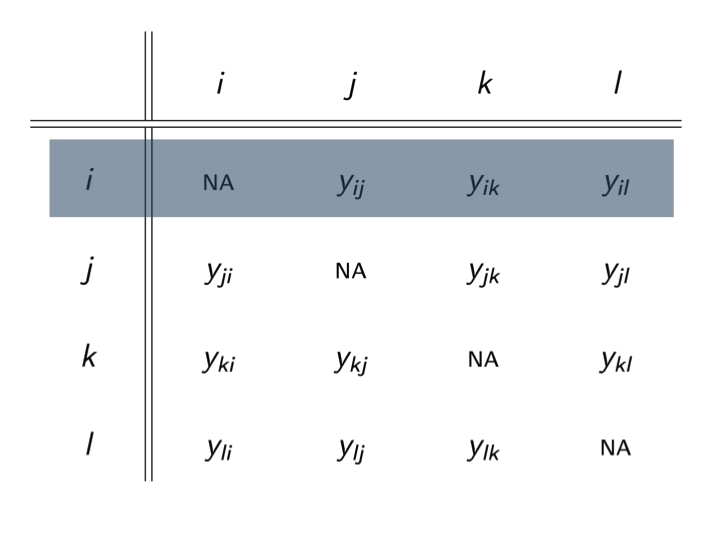
\includegraphics[width=.4\textwidth]{adjRowDep.png} & 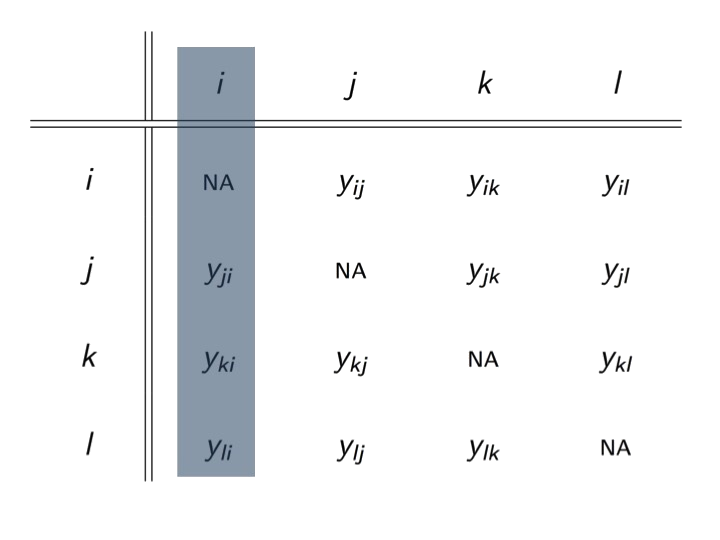
\includegraphics[width=.4\textwidth]{adjColDep.png} \\
		\textsc{Sender-Receiver Covariance} & \textsc{Reciprocity} \\
		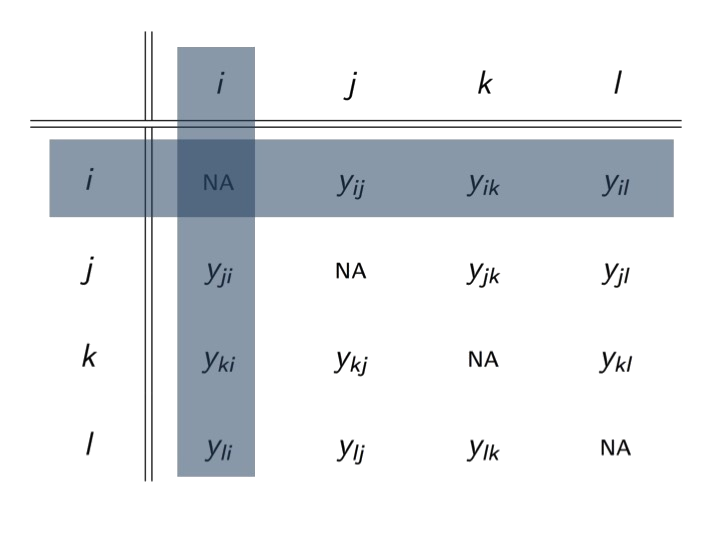
\includegraphics[width=.4\textwidth]{adjRowColCovar.png} & 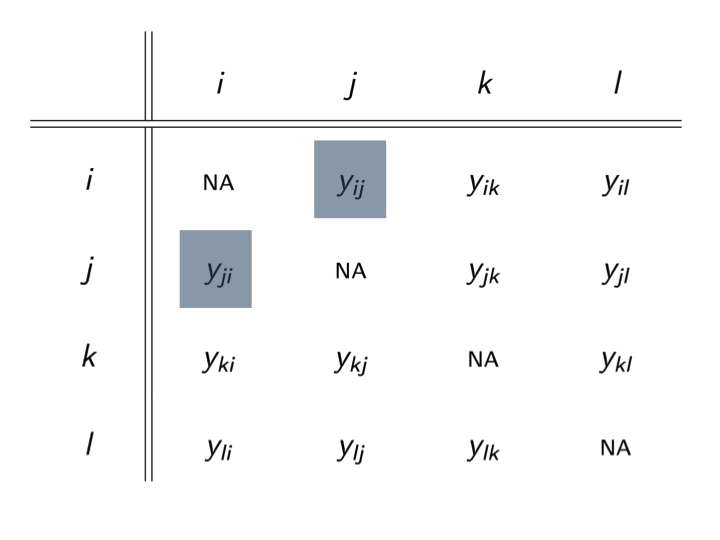
\includegraphics[width=.4\textwidth]{adjRecip.png} \\
	\end{tabular}
	\caption{Nodal and dyadic dependencies in relational data.}
	\label{fig:adjMatDeps}
\end{figure}

For similar reasons one also needs to take into account the shared dependence between observations that share a common receiver. The bottom-left panel in Figure~\ref{fig:adjMatDeps} illustrates that sender and receiver type dependencies can also blend together. Specifically, actors who are more likely to send ties in a network tend to also be more likely to receive them. As a result, the rows and columns in an adjacency matrix are often correlated. For example, consider trade flows both from and to many wealthy, developed countries. The bottom-right panel highlights a second-order dependence, specifically, reciprocity. This is a dependency occurring within dyads involving the same actors whereby values of $y_{ij}$ and $y_{ji}$ are correlated. The concept of reciprocity has deep roots in the study of relations between states \citep{richardson:1960,keohane:1989}.

For most relational data, however, dependencies do not simply manifest at the nodal or dyadic level. More often we find significant evidence of higher-order structures that result from dependencies between multiple groups of actors. These dependencies arise because there may be some set of latent attributes between actors that affects their probability of interacting with one another \citep{zinnes:1967,wasserman:faust:1994}. In Figure~\ref{fig:thirdDeps} we provide a visualization of a simulated relational dataset wherein the nodes designate actors and edges between the nodes indicate that an interaction between the two took place. To highlight third-order dependence patterns, nodes with similar latent attributes are colored similarly.

\begin{figure}[ht]
	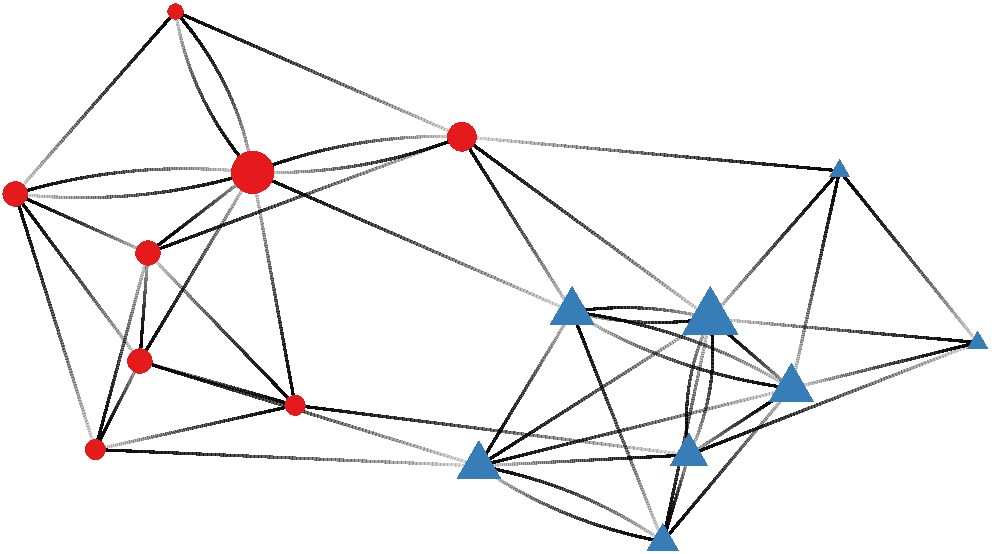
\includegraphics[width=.6\textwidth]{stochEquiv_v2.pdf}
	\caption{Visualization of a network with higher-order dependence patterns.}
	% need a simpler caption here
	\label{fig:thirdDeps}
\end{figure}

The visualization illustrates that the actors belonging to the same group have a higher likelihood of interacting with each other, whereas interactions across groups are rarer. A prominent example of a network with this type of structure is discussed by \citet{adamic:glance:2005}, who visualize linkages between right and left leaning political blogs preceding the 2004 United States Presidential Election. \citeauthor{adamic:glance:2005} find that the degree of interaction between right and left leaning blogs was minimal, and that most blogs were linked to others that were politically similar. This showcases the types of higher-order dependencies that can emerge in relational data. First, the fact that interactions were determined by a shared attribute, in this case political ideology, is an example of \textit{homophily}. Homophily explains the emergence of patterns such as transitivity (``a friend of a friend is a friend'') and balance (``an enemy of a friend is an enemy''), which also have a long history in international relations. The other major type of meso-scopic features that emerge in relational data is community structure \citep{mucha:etal:2010}, which is often formalized through the concept of stochastic equivalence \citep{anderson:etal:1992}. Stochastic equivalence refers to a type of pattern in which actors can be divided into groups such that members of the same group have similar patterns of relationships. In the example we have laid out above, each of the left leaning blogs would be considered stochastically equivalent to one another because any given left-leaning blog is more likely to interact with a blog of a similar political position and less likely to interact with one with a divergent political position.

These types of patterns frequently emerge in IR contexts as well.\footnote{For example, see: \citet{manger:etal:2012, kinne:2013, chyzh:2016}.} For example, a perennial finding in the interstate trade literature emphasizes the role that geography plays in determining trade flows. Geographic proximity in the network context is an example of a shared attribute between actors that corresponds to a greater likelihood of the event of interest taking place. Alternatively, in the interstate conflict literature, we may find that actors who are each a member of a particular (formal or informal) alliance are likely to act similarly in the conflict network. Specifically, they will tend to initiate conflictual events with actors that their fellow alliance members initiate conflict with, and they will be unlikely to initiate conflict with members of their alliance. In both these examples, we are able to explicitly parameterize the attribute that might explain the emergence of higher order dependence patterns, but it is likely that at times we will not able to account for the variety of reasons why higher order dependence patterns in networks may develop. 

% International Trade, we might observe homophily wherein states with open economies and an absence of Non-Tariff Barriers are more likely to trade with each-other all else equal; alternatively we might observe heterophily in the sense that states that have greater endowments of capital are more likely to trade with states with greater endowments of land or labor.

%  We would also likely observe stochastic equivalence in an interstate war network wherein countries who are in conflict with the same target country are unlikely to fight one another. In this case, countries with (formal or informal) alliances are a member of the same group due to similar conflictual ties to other actors in the system.

\section{\textbf{Additive and Multiplicative Effect Models for Networks}}

To account for the dependencies that are prevalent in dyadic data, we turn to the AME model. The AME approach can be used to conduct inference on cross-sectional and longitudinal networks with binary, ordinal, or continuous linkages. It is flexible and easy to use for analyzing the kind of relational data often found in social science. It accounts for nodal and dyadic dependence patterns, as well as higher-order dependencies such as homophily and stochastic equivalence.\footnote{\citet{minhas:etal:2016:arxiv} detail how this framework contrasts with alternative network-based approaches.} The AME model combines the social relations regression model (SRRM) to account for nodal and dyadic dependencies and the latent factor model (LFM) for third-order dependencies.  For details on the SRRM see \citet{li:loken:2002,hoff:2005,dorff:minhas:2017}.\footnote{An earlier version of the LFM  used in AME is presented as the general bilinear mixed effects (GBME) model in \citet{hoff:ward:2004}. The GBME model is more limited in the types of dependence patterns that it can capture due to the formulation of the matrix decomposition procedure.} The AME model is specified as follows:

\begin{align}
	\begin{aligned}
		y_{ij} \;=\; f(\theta_{ij}) &\text{, where } \\
		\theta_{ij} \;=\;& \bm\beta_{d}^{\top} \mathbf{X}_{ij} + \bm\beta_{s}^{\top} \mathbf{X}_{i} + \bm\beta_{r}^{\top} \mathbf{X}_{j} \text{\qquad(Exogenous parameters)} \\
		& + a_{i} + b_{j} + \epsilon_{ij} \text{\qquad\qquad\qquad\quad(SRRM parameters)} \\
		& + \mathbf{u}_{i}^{\top} \mathbf{D} \mathbf{v}_{j}  \text{\qquad\qquad\qquad\qquad\qquad\;(LFM parameters)} \\ 
	\label{eqn:ame}
	\end{aligned}
\end{align}

where $y_{ij,t}$ captures the interaction between actor $i$ (the sender) and $j$ (the receiver). We use a Bayesian probit framework, in which we model a latent variable, $\theta_{ij}$, using first a set of exogenous dyadic ($\bm\beta_{d}^{\top} \mathbf{X}_{ij}$), sender ($\bm\beta_{s}^{\top} \mathbf{X}_{i}$), and receiver covariates ($\bm\beta_{r}^{\top} \mathbf{X}_{j}$). Next, to account for the dependencies that emerge in dyadic data and that may complicate inference on the parameter associated with exogenous covariates, we add parameters from the SRRM and LFM. $a_{i}$ and $b_{j}$ in Equation~\ref{eqn:ame} represent sender and receiver random effects incorporated from the SRRM framework:

\begin{align}
	\begin{aligned}
		\{ (a_{1}, b_{1}), \ldots, (a_{n}, b_{n}) \} &\simiid N(0,\Sigma_{ab}) \\ 
		\{ (\epsilon_{ij}, \epsilon_{ji}) : \; i \neq j\} &\simiid N(0,\Sigma_{\epsilon}), \text{ where } \\
		\Sigma_{ab} = \begin{pmatrix} \sigma_{a}^{2} & \sigma_{ab} \\ \sigma_{ab} & \sigma_{b}^2   \end{pmatrix} \;\;\;\;\; &\Sigma_{\epsilon} = \sigma_{\epsilon}^{2} \begin{pmatrix} 1 & \rho \\ \rho & 1  \end{pmatrix}
	\label{eqn:srm}
	\end{aligned}
\end{align}

The sender and receiver random effects are modeled jointly from a multivariate normal distribution to account for correlation in how active an actor is in sending and receiving ties. Heterogeneity in the the sender and receiver effects is captured by $\sigma_{a}^{2}$ and $\sigma_{b}^{2}$, respectively, and $\sigma_{ab}$ describes the linear relationship between these two effects (i.e., whether actors who send [receive] a lot of ties also receive [send] a lot of ties). Beyond these first-order dependencies, second-order dependencies are described by $\sigma_{\epsilon}^{2}$ and a within dyad correlation, or reciprocity, parameter $\rho$. 

The LFM contribution to the AME is in the multiplicative term: $\mathbf{u}_{i}^{\top} \mathbf{D} \mathbf{v}_{j}=\sum_{k \in K} d_{k} u_{ik} v_{jk}$. $K$ denotes the dimensions of the latent space. The construction of the LFM here is actually quite similar to the recommender systems that companies like Amazon and Netflix have used to model customer behavior \citep{resnick:varian:1997,bennett:etal:2007}. This model posits a latent vector of characteristics $\mathbf{u_{i}}$ and $\mathbf{v_{j}}$ for each sender $i$ and receiver $j$. The similarity or dissimilarity of these vectors will then influence the likelihood of activity, and provides a representation of third-order interdependencies. The LFM parameters are estimated by a process similar to computing the singular value decomposition (SVD) of the observed network. When computing the SVD we factorize our observed network into the product of three matrices: $\mathbf{U}, \mathbf{D}, \text{ and }, \mathbf{V}$. This provides us with a low-dimensional representation of our original network.\footnote{The dimensions of $\mathbf{U}$ and $\mathbf{V}$ are $n \times K$ and $\mathbf{D}$ is a $K \times K$ diagonal matrix.} Values in $\mathbf{U}$ provide a representation of how stochastically equivalent actors are as senders in a network or, for example, how similar actors are in terms of who they initiate conflict with. $\hat{\mathbf{u}}_{i} \approx \hat{\mathbf{u}}_{j}$ would indicate that actor $i$ and $j$ initiate battles with similar third actors. $\mathbf{V}$ provide a similar representation but from the perspective of how similar actors are as receivers. The values in $\mathbf{D}$, a diagonal matrix, represent levels of homophily in the network.\footnote{Unlike traditional SVD, in the latent factor model, the singular values are not restricted to be positive, thus allowing us to account for both positive and negative homophily.} 

Note that this model easily generalizes to the case, common in IR, where interactions are undirected (for example the presence of conflict or a bilateral investment treaty). In the case of the SRRM, $\rho$ is constrained to be one and instead of separate sender and receiver random effects a single actor random effect is utilized. For the LFM, an eigen-decomposition scheme is used to capture higher order dependence patterns. In the application section, we show the applicability of the AME approach to both directed and undirected dyadic data.

By integrating the SRRM and LFM into a Bayesian probit framework, we can account for the underlying structure in dyadic data that, if left un-estimated, would complicate any inferences we might wish to draw for the exogenous parameters. Parameter estimation in the AME takes place within the context of a Gibbs sampler in which we iteratively sample from the posterior distribution of the full conditionals for each parameter. Specifically, given initial values of $\{\bm\beta, \mathbf{a}, \mathbf{b}, \mathbf{U}, \mathbf{V}, \Sigma_{ab}, \rho, \text{ and } \sigma_{\epsilon}^{2}\}$, the algorithm proceeds as follows until convergence:

 \begin{itemize}
 	\item sample $\bm\theta \; | \;  \bm\beta, \mathbf{X}, \bm\theta, \mathbf{a}, \mathbf{b}, \mathbf{U}, \mathbf{V}, \Sigma_{ab}, \rho, \text{ and } \sigma_{\epsilon}^{2}$ (Normal)
 	\item sample $\bm\beta \; | \;  \mathbf{X}, \bm\theta, \mathbf{a}, \mathbf{b}, \mathbf{U}, \mathbf{V}, \Sigma_{ab}, \rho, \text{ and } \sigma_{\epsilon}^{2}$ (Normal)
 	\item sample $\mathbf{a}, \mathbf{b} \; | \; \bm\beta, \mathbf{X}, \bm\theta, \mathbf{U}, \mathbf{V}, \Sigma_{ab}, \rho, \text{ and } \sigma_{\epsilon}^{2}$ (Normal)
	\item sample $\Sigma_{ab} \; | \; \bm\beta, \mathbf{X}, \bm\theta, \mathbf{a}, \mathbf{b}, \mathbf{U}, \mathbf{V}, \rho, \text{ and } \sigma_{\epsilon}^{2}$ (Inverse-Wishart)
 	\item update $\rho$ using a Metropolis-Hastings step with proposal $p^{*} | p  \sim$ truncated normal$_{[-1,1]}(\rho, \sigma_{\epsilon}^{2})$
 	\item sample $\sigma_{\epsilon}^{2} \; | \; \bm\beta, \mathbf{X}, \bm\theta, \mathbf{a}, \mathbf{b}, \mathbf{U}, \mathbf{V}, \Sigma_{ab}, \text{ and } \rho$ (Inverse-Gamma)
 	\item For each $k \in K$:
 	\begin{itemize}
 		\item Sample $\mathbf{U}_{[,k]} \; | \; \bm\beta, \mathbf{X}, \bm\theta, \mathbf{a}, \mathbf{b}, \mathbf{U}_{[,-k]}, \mathbf{V}, \Sigma_{ab}, \rho, \text{ and } \sigma_{\epsilon}^{2}$ (Normal)
 		\item Sample $\mathbf{V}_{[,k]} \; | \; \bm\beta, \mathbf{X}, \bm\theta, \mathbf{a}, \mathbf{b}, \mathbf{U}, \mathbf{V}_{[,-k]}, \Sigma_{ab}, \rho, \text{ and } \sigma_{\epsilon}^{2}$ (Normal)
 		\item Sample $\mathbf{D}_{[k,k]}  \; | \; \bm\beta, \mathbf{X}, \bm\theta,\mathbf{a}, \mathbf{b}, \mathbf{U}, \mathbf{V}, \Sigma_{ab}, \rho, \text{ and } \sigma_{\epsilon}^{2}$ (Normal)\footnote{Subsequent to estimation, $\mathbf{D}$ matrix is absorbed into the calculation for $\mathbf{V}$ as we iterate through $K$. }
 	\end{itemize}
 \end{itemize}

The presence of these dependencies in relational data points to the fact that there is a complex structure underlying the dyadic events that we observe, and that accounting for this structure is necessary if we are to adequately represent the data generating process. Of course, if one can specify each of the nodal, dyadic, and triadic set of attributes that influence interactions then the conditional independence assumption underlying standard approaches will be satisfied. However, it is rarely the case that this is possible even for TSCS data and thus modeling decisions must account for underlying structure. Failing to account for the underlying structure in either TSCS or dyadic data leads to a number of well-known challenges: a) biased estimates of the effect of independent variables, b) uncalibrated confidence intervals, and c) poor predictive performance. Additionally, by ignoring these potential interdependencies, we often ignore substantively interesting features of the problem. The study of international relations is founded on the relations among actors. Why ignore the interdependencies that led to the study of IR in the first place?
\section{Simulation study}

We use a simulation study to highlight the ability of AME to conduct inference on exogenous parameters in the presence of network dependencies. We are particularly interested in whether the LSM can adjust for confounding when the confounding variable is unmeasured. In the simulation design, we study how the level of confounding affects the performance of AME relative to the GLM. We evaluate performance in terms of bias and inferential error. For simplicity and computational efficiency we consider a unidimensional latent space. 

Here we consider inference for a regression parameter $\beta$ of a linear or generalized linear model for a network in the case where there is an omitted variable. The true data-generating models we consider are of the form 

$y_{i,j} \sim  \mu + \beta x_i x_j + \gamma w_i w_j + \epsilon_{i,j} $

where $Y= \{y_{i,j}\}\in \mathbb R^{n\times n}$ is an observed sociomatix, $x = \{x_i \} \in \mathbb R^n$ is a vector of observed node-specific characteristics, and $w = \{ w_i\} \in \mathbb R^n$ is a vector of unobserved node-specific characteristics. We compare inference for $\beta$ using three models:

\begin{itemize}
	\item A naive regression model assuming independent errors; 
	\item A latent factor model; 
	\item An ``oracle'' regression model that includes both $x_{i,j}=x_i x_j$ and $w_{i,j}=w_i w_j$. 
\end{itemize}

We make these comparisons in the context of a binary network outcome with a probit regression model. 

One way to compare inferences across models is  with bias and variance of the parameter estimates. Both of these quantities are combined to get the MSE. 

Alternatively, bias and precision can be summarized by confidence interval coverage and width. Coverage should ideally be at the nominal level. If two methods have the same actual coverage rate, the one with the narrower intervals is preferred. 

\begin{figure}
	\centering
	\caption{Bias in parameter when homophily is ignored.}
	\label{fig:ameBias}
	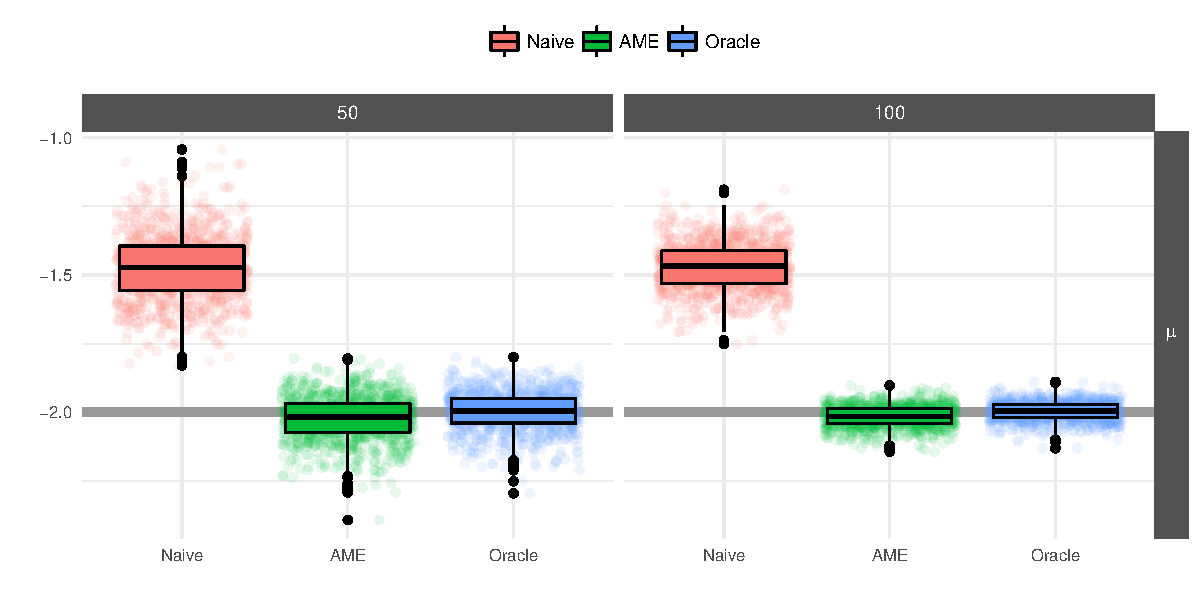
\includegraphics[width=1\textwidth]{ameSimBias_mu.pdf} \\
	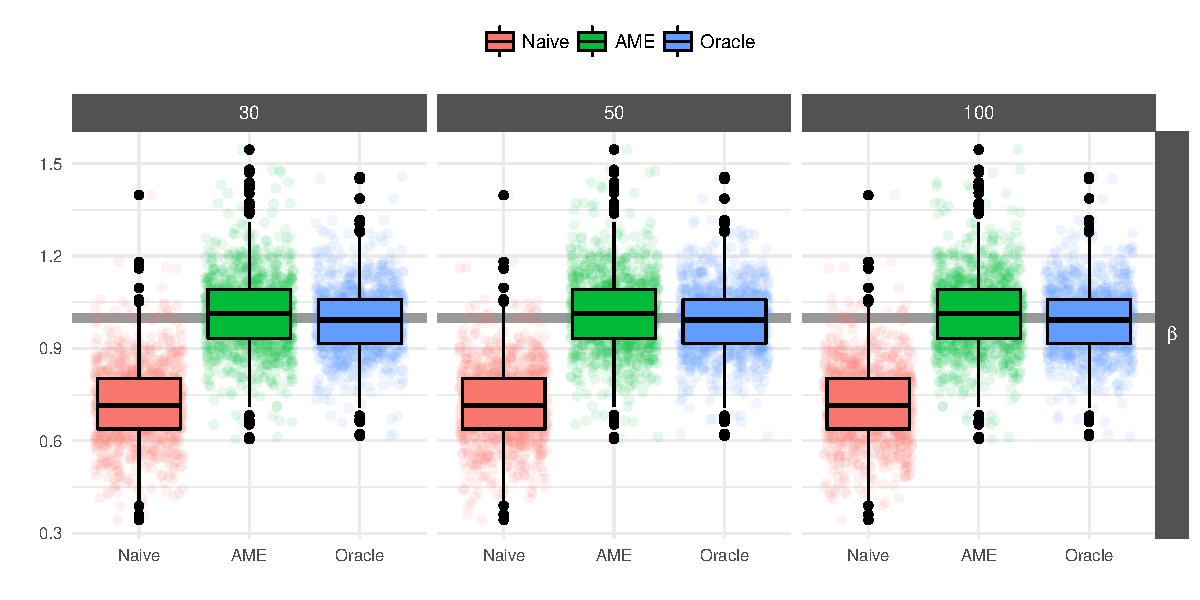
\includegraphics[width=1\textwidth]{ameSimBias_beta.pdf}
\end{figure}

\begin{figure}
	\centering
	\caption{Coverage in parameter when homophily is ignored.}
	\label{fig:ameCalib}
	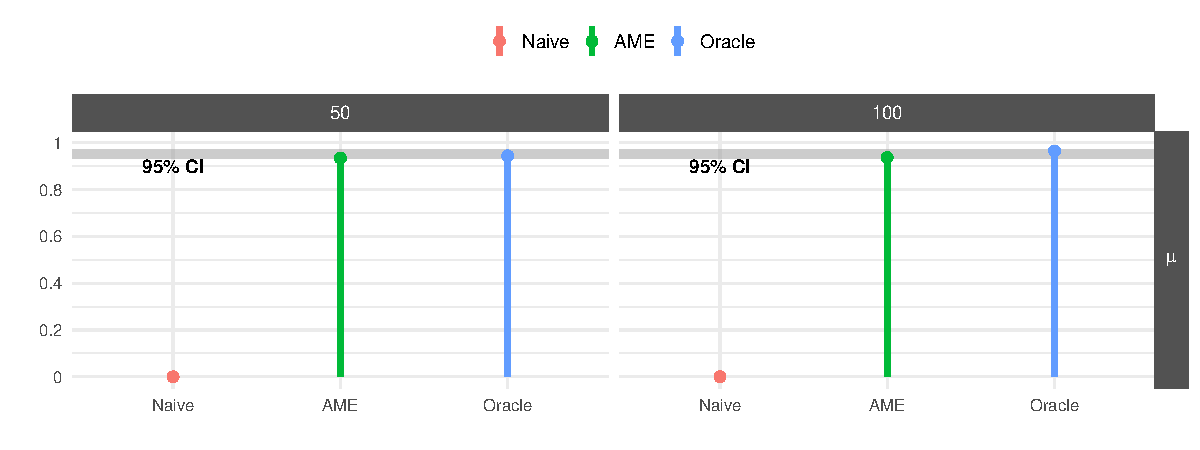
\includegraphics[width=1\textwidth]{ameSimCover_mu.pdf} \\
	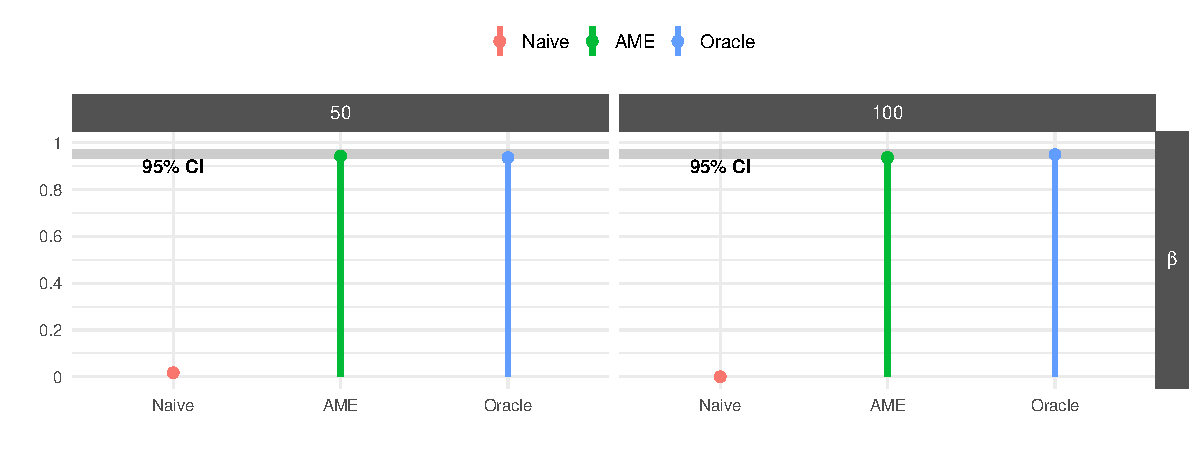
\includegraphics[width=1\textwidth]{ameSimCover_beta.pdf}
\end{figure}

\begin{figure}
	\centering
	\caption{Correlation between missing variable and multiplicative random effect in AME.}
	\label{fig:ameCorr}
	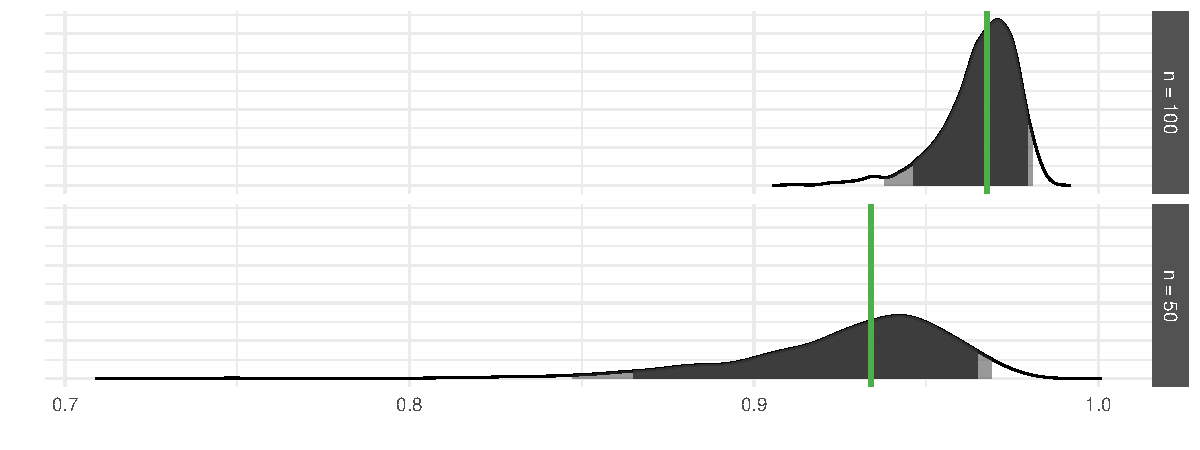
\includegraphics[width=1\textwidth]{ameSimCorr.pdf} \\
\end{figure}

\section{Replications}
 
\subsection{Design}

We choose five prominent studies from the broad field of international relations and international political economy that utilize relational data \citep{reiter:stam:2003, mcdonald:2004,  rose:2004, weeks:2012, gibler:2017}. These studies are recent and have been cited over 100 times. Each of these pieces was published in a prominent journal and is well-known in the literature. Each used the standard approach in political science, which is to employ some form of a general linearized regression that ignores dyadic interdependencies, except as they may reveal themselves in included variables. Also part of the gold standard is a post estimation cleanup thought to be a paliative, and each of these studies adjust the posterior standard errors in an attempt to account for the clustering of observations.

\begin{table}
\caption{Features of the Studies Replicated. }
	\begin{tabular}{lcccccc}
& Model & N. Actors & Years  & N. Dyads & Dyads Type & Clustering $\sigma_{\hat{\beta}}$ \\ \toprule
Reiter \& Stam (2003) & Logit & & & $753,456$ & Directed & Robust \\	McDonald (2004) & Logit & & & $92,354$ & Undirected & Robust\\
Rose (2004) & OLS & ? &  ?& $234,597$ & Directed & Robust \\	 
Weeks (2012) & Logit & ? & ?& $901,540$ & Directed & Robust \\
Gibler (2017) & Logit & 21,275 & 193 & $650,557$ & UnDirected & no \\ \bottomrule
	\end{tabular}
\end{table}

We obtained the data for each of these studies from their replication archives and replicated the main results of each of the articles.\footnote{Without exception this was straightforward to accomplish, thanks to an increasing norm in the social sciences of open data sharing.} We also examine each of the models using the AME framework described above.  Our goal is to ascertain whether the ignored interdependencies---the non-iid structure of the relational data---would result in different model estimates when they were addressed in an AME framework, and more importantly to see if there were substantive opportunities that were presented with the dynamic factor approach.  

Finally, in each study we assess whether there is any new substantive finding that emerges or indeed if any disappear once the interdependencies in the data are modeled.

The broader goal, beyond introducing the use of the AME framework in an applied setting, is to examine the extent to which interdependencies within typical dyadic data make much difference in what we have learned about international relations from recent empirical studies that use a framework that ignores dependencies.  We believe that it does, and that the dynamic latent factor model provides a step forward.

Given current practices, most scholars have a single variable in a complicated empirical model that they look at for evaluating the validity of their empirically estimated models.  Whether putative control variables, for example, are precisely estimated is less important. Generally, interpretations focus on a small set of independent variables.  In the study by Reiter and Stam (2003) the main question is to determine in mixed dyads---consisting of a democratic country and country ruled by a personalist dictatorship---whether it is the
democratic country or the personalist country that is associated with a greater likelihood that the dyad is in a dispute.  In a regression including fourteen coefficients, they focus on whether the variables that capture whether the initiator is a democratic country are statistically significant.\footnote{In particular, the variables \texttt{Pers/Democ} and \texttt{Democ/Pers} in Model 3, in Table 1, page 335.} In our evaluation we focus on the same question in the re-examination of the Reiter and Stam study to determine whether the model replicates when reestimated within the AME framework. Each of the other four studies also has a crucial finding that we hone in on to further draw into focus the potential differences brought about by utilizing an AME estimation procedure.  In Table~\ref{tab:modelFindingSumm}, we present the overall results; the term \textbf{fails to replicate} indicates only that the sign and/or significance of the crucial finding in the original study is not also found in the AME estimation.
 

\begin{table}[ht]
\centering
\caption{Here we provide a brief summary of the key variable in each of the five replications and a note about whether or not the finding is replicated when using our network based approach. Cases in which the substantive finding is not replicated are highlighted in bold.}
\begin{tabular}{l p{7cm} l} \toprule
\multirow{2}{*}{Study} & \multirow{2}{*}{Central Finding} & Does it Replicate \\ 
	& &  in a Network Model? \\ \toprule
Reiter \& Stam (2003) & Personalist Regimes Attack Democracies, Not Vice Versa & Replicates \\ \midrule
McDonald (2004) & Lower Trade Barriers and Higher Trade Lead to Peace & \textbf{Fails to Replicate} \\ \midrule
Rose (2004) & WTO Membership Does not Effect Trade & Replicates \\ \midrule
Weeks (2012) & Bosses, Juntas and Strongmen are more Aggressive, Machines are Not & \textbf{Fails to Replicate} \\\midrule
Gibler (2017) & Power Parity at Time of Entry to International System Inceases Conflict & \textbf{Fails to Replicate} \\ \bottomrule
	\end{tabular}
			\label{tab:modelFindingSumm}
\end{table}

In addition, we also examine the predictions made with each approach using an out-of-sample cross validation strategy. By accounting for exogenous and network dependent patterns that give rise to conflict systems we are able to better account for the data generating process underlying relational data structures. To show that this is the case, we examine whether our approach achieves better predictive performance in an out-of-sample context than traditional dyadic models. To evaluate our model, we randomly divide the $\binom n 2 \times T$ data values into $k=30$ sets, letting $s_{ij,t}$ be the set to which pair $ij,t$ is assigned. Then for each $s \in \{1,\ldots,k\}$, we:

\begin{enumerate}
	\item estimate model parameters with $\{y_{ij,t}: s_{ij,t} \neq s\}$, the data not in set $s$,
	\item and predict $\{\hat{y}_{ij,t}: s_{ij,t} = s\}$ from these estimated parameters. 
\end{enumerate}

\noindent The result of this procedure is a set of sociomatrices $\bm \hat Y$, in which each entry $\hat y_{ij,t}$ is a predicted value obtained from using a subset of the data that does not include $y_{ij,t}$. 

We set a number of benchmarks for comparison. First, we compare the AME model to a GLM model (that used in the original study) using the same covariates to show the effect of accounting for network dependencies on predicting conflict. We supplement this with an alternative GLM that includes not just these covariates, but also a lagged dependent variable and a lagged reciprocity term. The lagged dependent variable is the equivalent of saying that conflict and peace are relatively likely to persist between dyads, while the inclusion of a lagged reciprocity term in a GLM framework is a simple way to account for retaliatory strikes.

We utilize three performance criterions to compare the models: Receiver Operator Characteristic (ROC) curves, Precision Recall (PR) curves, and separation plots. ROC curves look at the trade-off between true positive rates and false positive rates at different thresholds of classification. An issue with an ROC Curve when looking at conflict, is that it is relatively rare at the dyadic level: in most years only 3\% of possible dyads are in conflict with one another. If peace is common, even a poor model will have a very low False Positive Rate. The ROC curves are best for balanced samples with as many events as non-events. To better assess which models predict the presence of conflict, not just its absence, we look at PR Curves. These examine the trade-offs between the percentage of conflicts a model predicts, and the percentage of predicted conflicts which occur. Lastly, we examine separation plots \citep{greenhill:etal:2011}. These provide an intuitive visualization of the accuracy of our predictions by juxtaposing a line showing the predicted probability of conflict with whether conflict actually occurs for all cases (where the cases are sorted by the predicted probability and then colored to indicate the outcome). Here a perfect model would have all cases where conflict actually exists on the right with a predicted probability of $1$, and would predict $0$ in all other cases. All of the models' performance out of sample by these metrics are displayed in figure \ref{fig:roc_ame}. The AME model with covariates is the best performing model out of sample in all cases. This model outperforms each of the GLM variants by a notable margin.
% % % % % % % % % % % % % % % % % % 

\begin{table}[ht]
\centering
	\begin{tabular}{l|l cc}
	~ & ~ & GLM & AME \\
	\toprule
\multirow{2}{*}{Reiter \& Stam (2003)} & AUC (ROC) & 0.92 & \textbf{0.96} \\
		~ & AUC (PR) & 0.08 & \textbf{0.15} \\		\midrule
\multirow{2}{*}{McDonald (2004)} & AUC (ROC) & 0.92 & \textbf{0.99} \\
		~ & AUC (PR) & 0.13 & \textbf{0.28} \\		\midrule
\multirow{2}{*}{Rose (2004)} & Root Mean Squared Error (RMSE) & 3.23 & \textbf{1.99} \\
		~ & Root Median Squared Error (RMDSE) & 2.01 & \textbf{1.06} \\	\midrule
\multirow{2}{*}{Weeks (2012)} & Area Under ROC Curve (AUC-ROC) & 0.64 & \textbf{0.97} \\
		~ & Area Under PR Curve (AUC-PR) & 0.00 & \textbf{0.15} \\		\midrule
\multirow{2}{*}{Gibler (2017)} & AUC (ROC) & 0.52 & \textbf{0.91} \\
		~ & AUC (PR) & 0.00 & \textbf{0.08} \\			\bottomrule
	\end{tabular}
	\caption{Here we provide a summary of the out-of-sample performance based on our cross-validation strategy for each of the five replications when using the standard dyadic approach and our network based approach. Four of the five studies involved a binary dependent variable, so for those measures we provide area under the curve (AUC) statistics. The Rose study involved a Gaussian dependent variable and for that we use the root mean squared error (RMSE) and root median squared error (RMDSE). Cases in which our network based approach outperformed the standard approach are highlighted in bold.}
	\label{tab:modelPerfSumm}
\end{table}
\FloatBarrier

%%% TO HERE
\subsection{Replication of Weeks (2012)}

\citet{weeks:2012} examines the influence of domestic institutions on the initiation of military conflicts by autocratic leaders.  She argues that in some circumstances autocrats are held accountable for their foreign policy decisions. She adds the nuance that autocratic audiences are not homogeneous. When the autocratic regime is nonmilitary, the domestic audience do not favor military actions, but in military autocracies this is not the case. Further she argues that in personalistic regimes without a military or civilian domestic audience, the leaders tend to be more likely to employ military force in their foreign policy.  To study this question, she uses a dyadic design in which the dependent variable is ``whether country A in a directed dyad initiated military conflict against country B during year t'' (page 337).  These data come from the Militarized Interstate Disputes database \citep{maoz:2005}.  One major innovation in her study resides in the nuanced way in which she conceptualized and coded regime type into four types: a) Machine, b) Junta, c) Boss, and d) Strongmen. She also includes a variety of putative control variables focusing on capabilities for both sides of the dyad, alliances, geography, trade dependence, regime instability, and the regime type of ``side B.''  She uses a logistic regression, but follows \citet{beck:etal:1998} and includes splines to capture temporal covariation in the dependent variable along with  fixed, unit effects. The analysis is done for dyads, but is considered to be from the perspective of the actor that initiated the dispute. Her time frame is from 1946-1999.  The basic finding is that a) juntas, bosses, and strongmen are more likely to initiate conflict than machines (and maybe democracies) and that b) machines are no more belligerent than democracies.  These insights are mainly determined by looking at coefficients and their putative significance in Tables 1 and 2 (pages 339--340). She makes the argument that ignoring important nuances between different types of autocracies hinders our understanding of the initiation of military conflict by autocracies. 

The replication of \citet{weeks:2012} likely has the sharpest divergence between the General Linear Model results and those of the AME Model. In Weeks's initial models,  she finds that machines are less prone to initiate conflict than the reference category, whereas Juntas, Bosses and Strong-men are more conflict-prone, in line with her theoretical expectations. When we look at the posterior distribution of these coefficients in the AME results, we find that none of these values are distinguishable from zero. We similarly find less pronounced effects for military capabilities. One explanation for this divergence is the AME model's ability to account for third order effects. Inspection of the multiplicative effects in Figure~\ref{fig:weekscirc} reveals a number of clusters of states which exhibit structural equivalence -- in the top right corner we see states like the US, the UK, and Israel who often send conflict to similar targets. In particular, we observe a cluster of ``rogue states,'' who are receivers of conflict, in the top right (Iran, Iraq, Syria, Libya, North Korea). In the bottom corner we see a cluster of authoritarian senders including Iraq, Russia, Syria, North Korea and China. In general, these clusters have similar governmental types (Iraq, Syria, Libya, and North Korea all fell under the ``boss" category), and similar conflict behavior. So, in the GLM, which ignores these third order dependencies, much of these results might have been attributed to regime type. The AME model, on the other hand, finds that it is more efficient to attribute this behavior to the multiplicative effects. In terms of out of sample performance, shown in Figure~\ref{fig:weeksauc}, the AME model performs markedly better than the GLM out of sample, lending credence to the possibility that these third order dependencies cause spurious effects for regime type.

\begin{figure}
	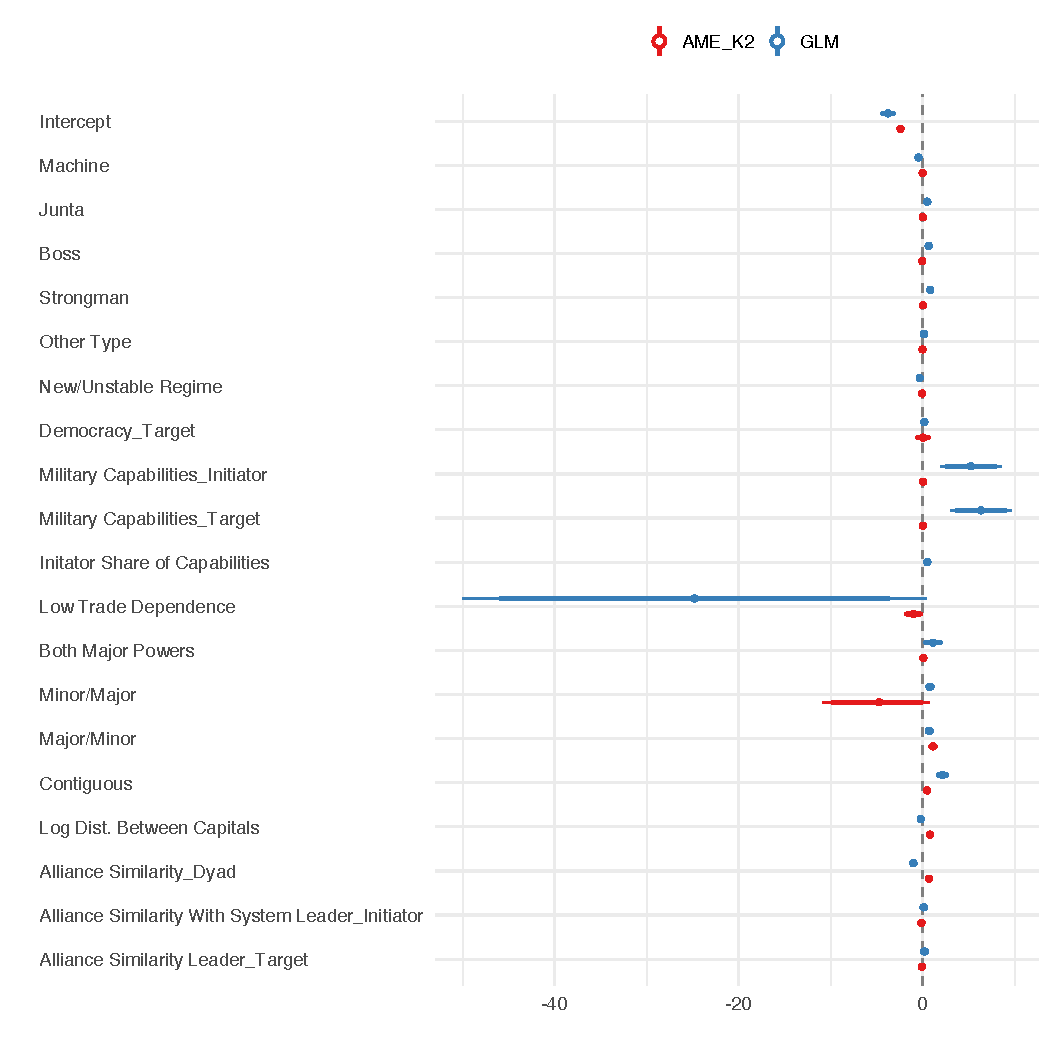
\includegraphics[width=\textwidth]{weeks_coefs_all.pdf}
	\caption{\label{fig:weeksCoef} Coefficient plot of Weeks' (2012) original model (blue) compared to AME model (red). }
\end{figure}

\begin{figure}
\centering   
	\subfigure[AUC]{\label{fig:weeksauc}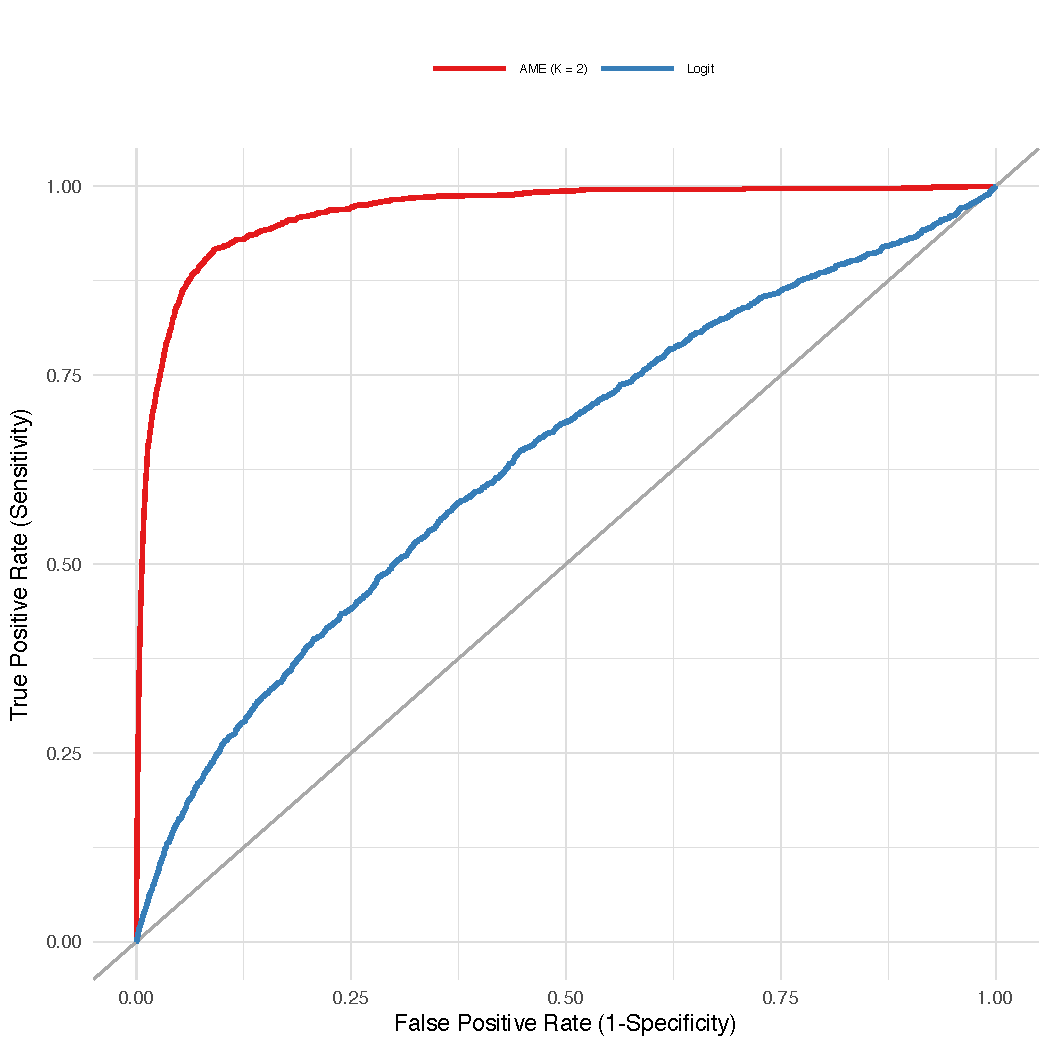
\includegraphics[width=65mm]{weeks_auc_outsamp.pdf}}
	\subfigure[Precision and Recall]{\label{fig:reitpr}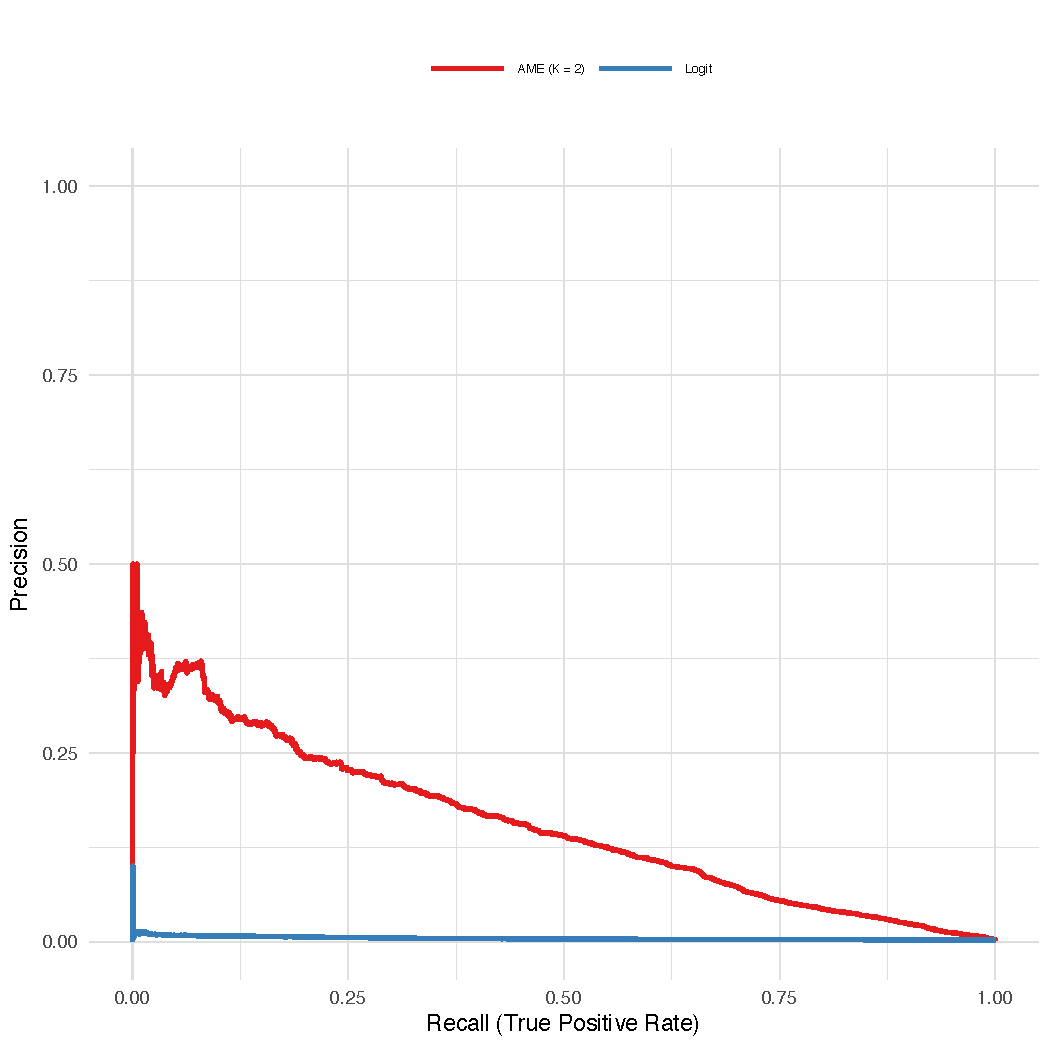
\includegraphics[width=65mm]{weeks_pr_outsamp.pdf}}
	\caption{Assessments of out-of-sample predictive performance for Weeks (2012) using ROC curves and PR curves.}
\end{figure}

\begin{figure}
	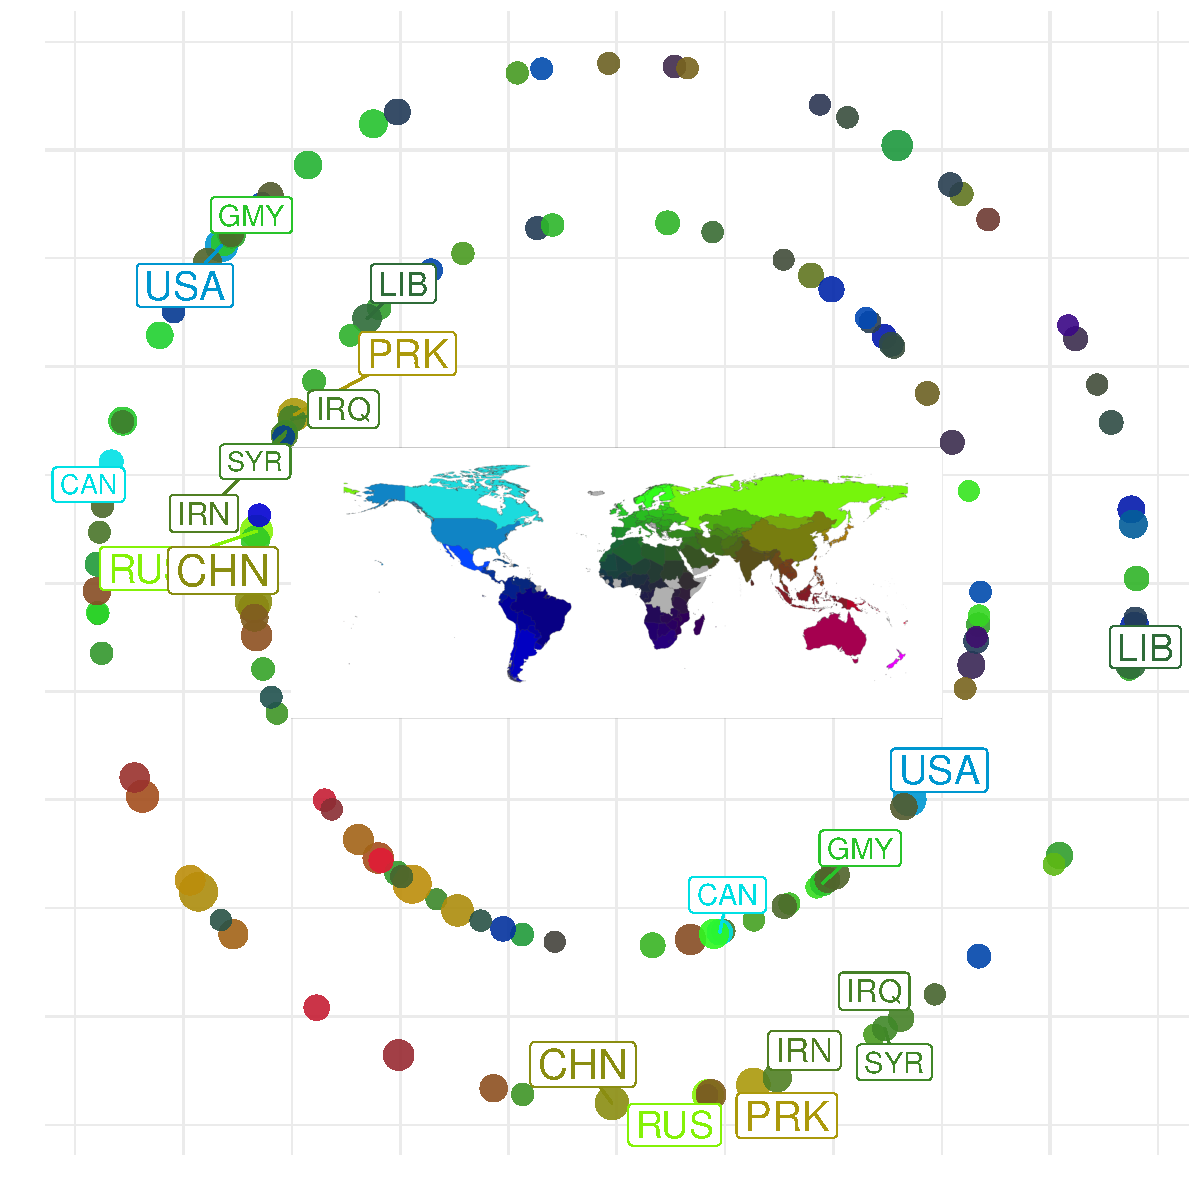
\includegraphics[width=\textwidth]{weeks_circPlot.pdf}
	\caption{\label{fig:weekscirc} Visualization of multiplicative effects for Weeks (2012). Blue represents groups with common sending patterns and red represents groups with common receiving patterns.}
\end{figure}

\subsection{Replication of Reiter \& Stam (2003)}

\citet{reiter:stam:2003} examine the relationship between democracy, dictatorship and the initiation of militarized disputes.  They use directed dyads and find that dyads involving a democratic leader on the one hand and a personalist dictator on the other tend to be violent. They also discover that dictators are likely to challenge democracies, but that this is not reciprocal.  In addition, military regimes and single-party regimes are more prone to initiate disputes with democracies, than the other way around.  They use the MID data, but note that ``We code a state as having initiated a dispute if it is on `side A' of a MID, the conventional approach to coding initiation. This means that the state was on the side that took the first action in the dispute, whether that action was the threat, display, or use of force. We code joiners as initiators or targets, though the results do not change if we do not code joiners as initiators or targets. \ldots Though coding initiation will always be difficult, the `side A' variable has been widely used in past conflict scholarship (page 334).'' Independent variables are largely taken from an earlier study and focus on various encodings of regime types, contiguity, alliance, and capability measures. As is prevalent in these kinds of studies, Reiter \& Stam employ a logistic regression that includes an indicator of the time since the last dispute as well as three cubic splines. The database for this study is constructed using EUGene \citep{bennett:stam:2000} and comprises approximately three-quarters of a million stacked dyads. Based on their statistical analysis, they conclude that institutional constraints affect the propensity of democratic and non-democratic leaders to engage in military conflict. 

In the original model, the variable ``Pers/Democ Directed Dyad" (which represents a Personalist $\rightarrow$ Democractic directed dyad) is clearly positive while the variable ``Democ/Personalist Directed Dyad'' is zero and the difference between the two coefficients is clearly distinct from zero. In our replication using the AME framework, we also find that Pers-Democ directed dyad has a positive effect with zero excluded from the 95\% confidence interval while Democ-Pers directed dyad is indistinguishable from zero. Using this model, however, we can no longer conclusively say that the Pers/Democratic coefficient is larger than the Democ/Personalist one.
Our replication using the AME approach therefore cast some doubt on Reiter \& Stam's key claim that MIDs initiated by personalist dictatorships against democracies are more likely than MIDS initiated by democracies. Further, the effect of most of the covariates in the literature thought to predict interstate MIDs are much closer to zero when using the AME framework. Finally, our modeling approach outperforms the original model by better, and more accurately, predicting MIDs out-of-sample (Figure~\ref{fig:reitaucpr} and Figure ~\ref{fig:reitpr}).  

\begin{figure}
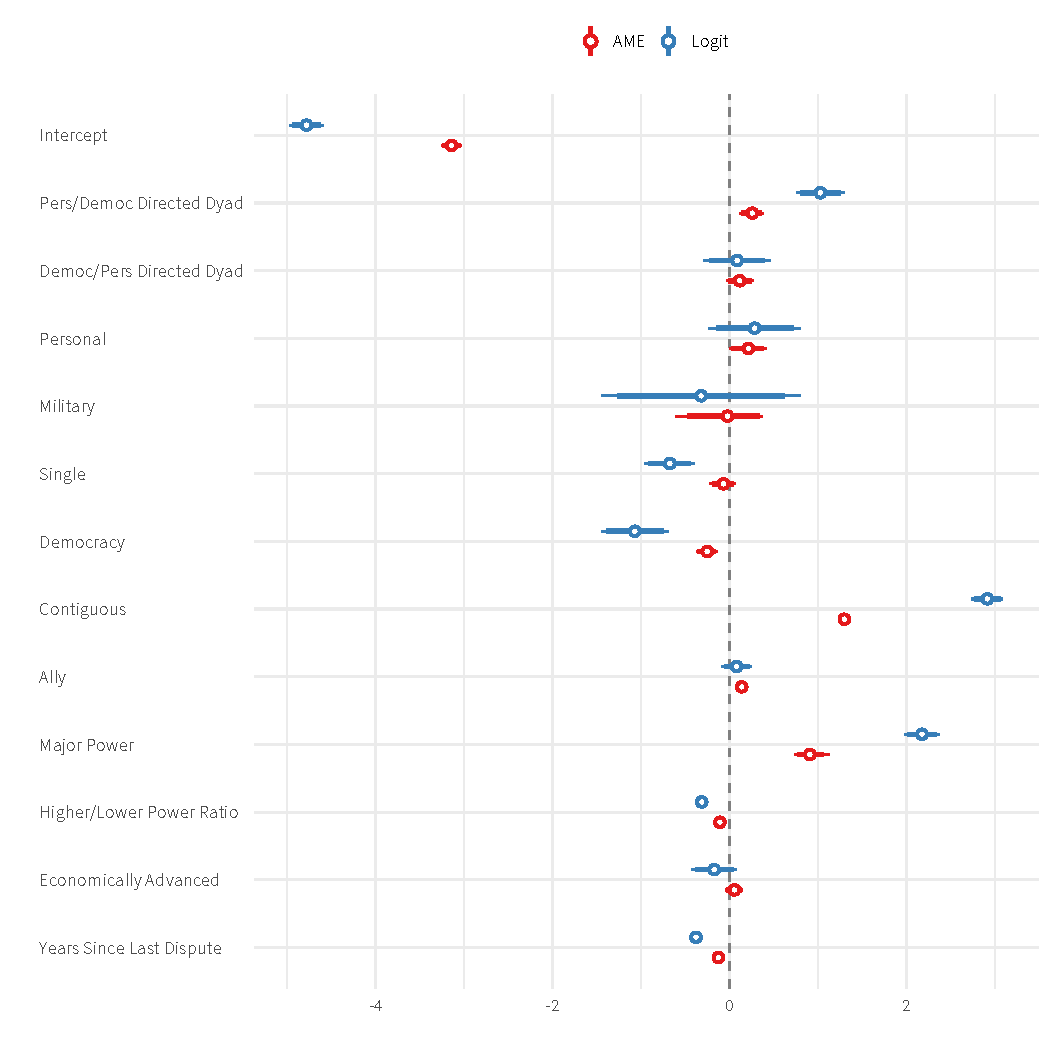
\includegraphics[width=\textwidth]{reiter_coefs_all.pdf}
\caption{\label{fig:reitCoef} Coefficient plot of Reiter \& Stam (2003)'s original model (blue) compared to AME model (red). }
\end{figure}

\begin{figure}
\centering   
\subfigure[AUC]{\label{fig:reitauc}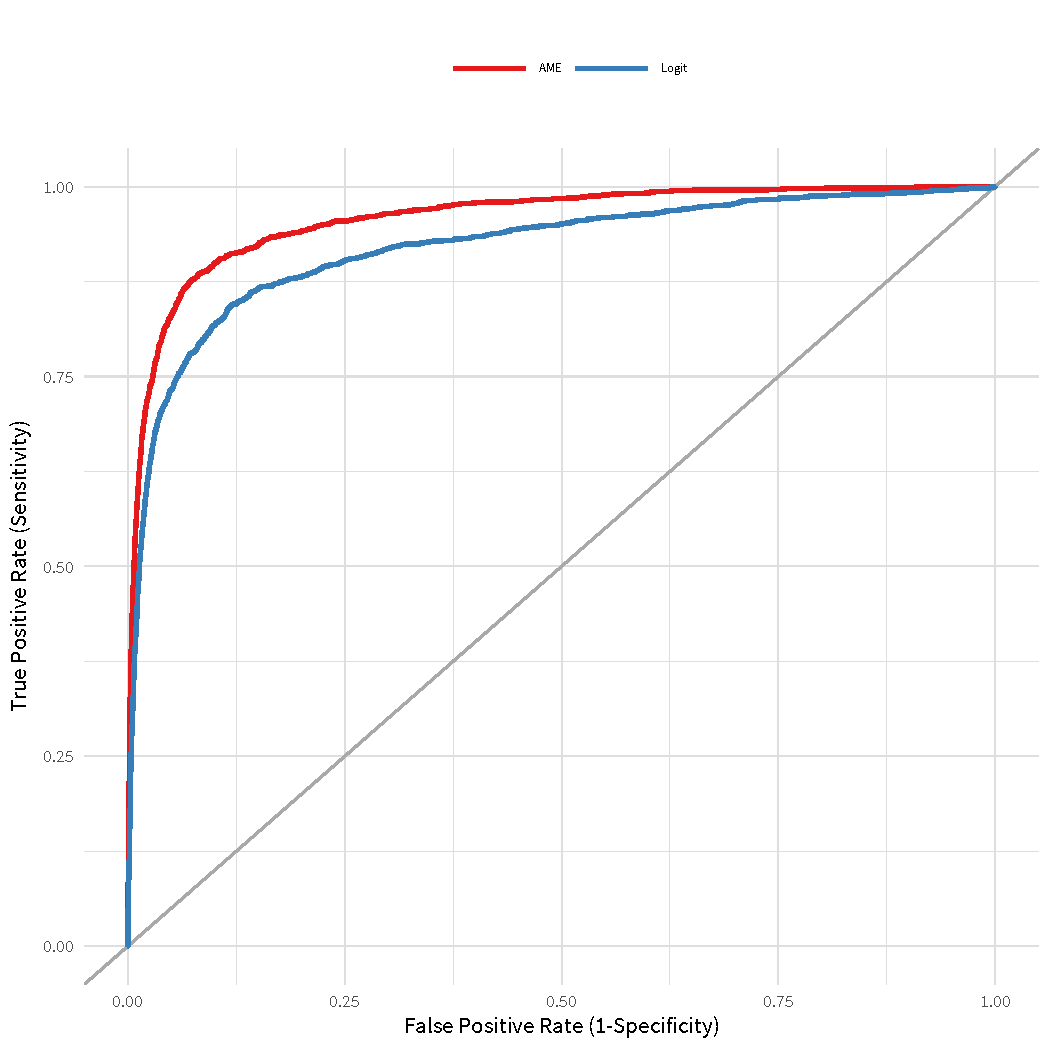
\includegraphics[width=65mm]{reiter_auc_outsamp.pdf}}
\subfigure[Precision and Recall]{\label{fig:reitpr}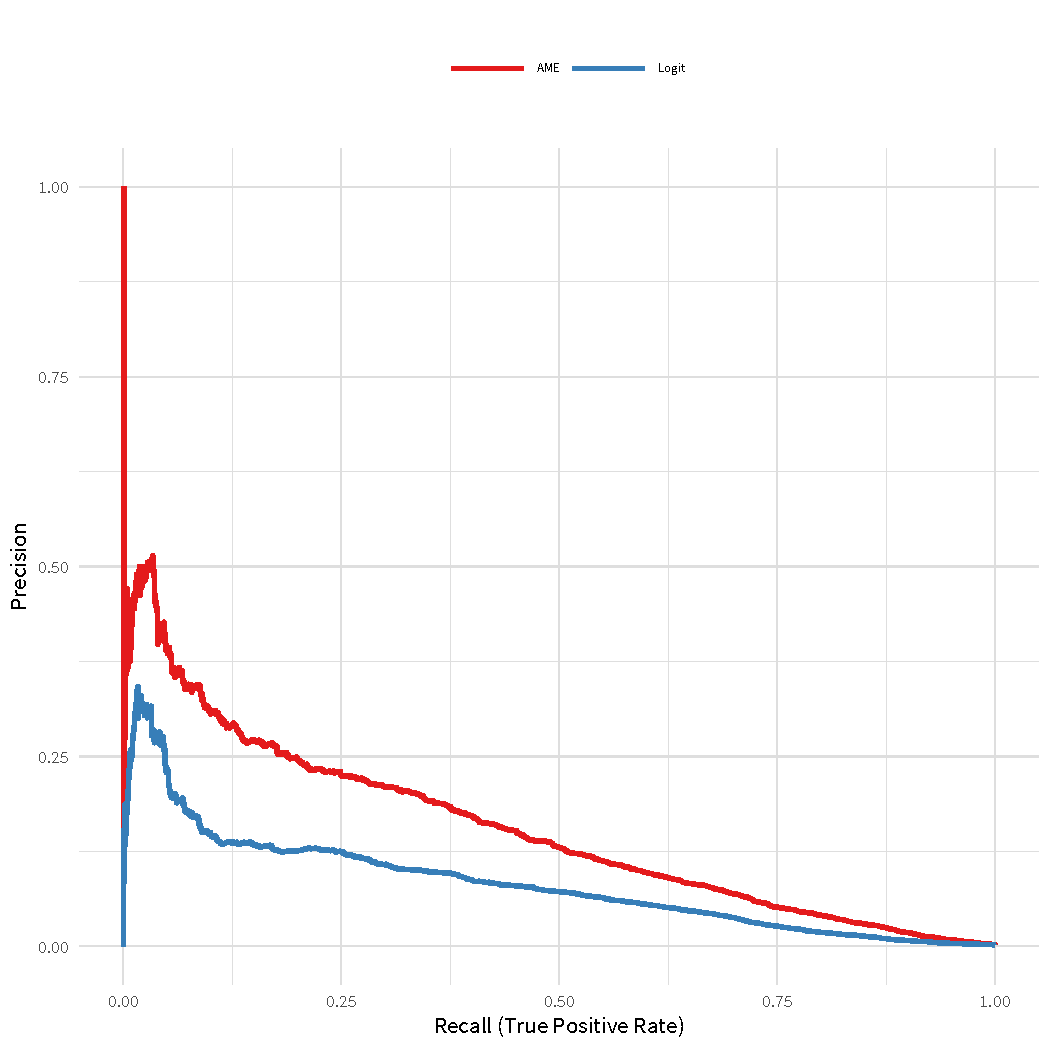
\includegraphics[width=65mm]{reiter_pr_outsamp.pdf}}
\caption{Assessments of out-of-sample predictive performance for Reiter \& Stam (2003) using ROC curves and PR curves.}
\end{figure}

\subsection{Replication of Rose (2004)}

In 2004, Andrew Rose published a study in the \textit{American Economic Review} \nocite{rose:2004} that proved to be quite controversial in terms of macroeconomic trade theory and in terms of trade policy in a variety of nations. It also provoked a number of responses in the international political economy literature \cite{tomz:etal:2007,ward:etal:2013}.  Rose's basic argument is that despite longstanding arguments made by trade theorists and the World Trade Organization that WTO membership fosters greater cooperation and thereby more trade among its members, the empirics do not bear out such claims. He uses a standard gravity model with dyadic data on bilateral merchandise trade (not services) for $175$ countries over a period of five decades. Estimating this model using OLS within many differing contexts, his conclusion was that: ``An extensive search reveals little evidence that countries joining or belonging to the GATT/WTO have different trade patters from outsiders... (2004, page 98, abstract).''  The data for this study have been widely used in replications by many searching for the missing effects of the WTO---as well as preferential trade agreements, bilateral investment theories, and other aspects of modern trade theory.  

When we compare the results of Rose's original OLS model to the AME model accounting for network dependencies, the results are generally similar. The main result of the model---the null effect of membership in the WTO, as represented by the ``One-In" and ``Both-In" variables---persists in the AME model. However, while in the original model there was a clear positive relationship between Real GDP and Trade, most of this effect vanishes in the AME model. The random effects shown in Figure~\ref{fig:roser} reveal the cause of much of this divergence. Here, the states with the most positive random effects are also states with high GDP, though not necessarily high GDP/capita.\footnote{Note: Qatar exhibits strongly negative random effects.} Thus, the effect of GDP in the original model was, in part, an artifact of first-order dependencies. Most of the other results of the model are constant across each model, though some geographic features, such as islands and landlocked states, have a more clear effect on trade once we account for these network dependencies. When we account for network interdependencies, we observe a markedly lower Root Mean Squared Error out-of-sample---$3.23$ for the OLS model and $1.77$ for the AME model. While the basic model replicates with the basic result, there are substantial and substantive improvements gleaned from the AME results.

%\begin{figure}
%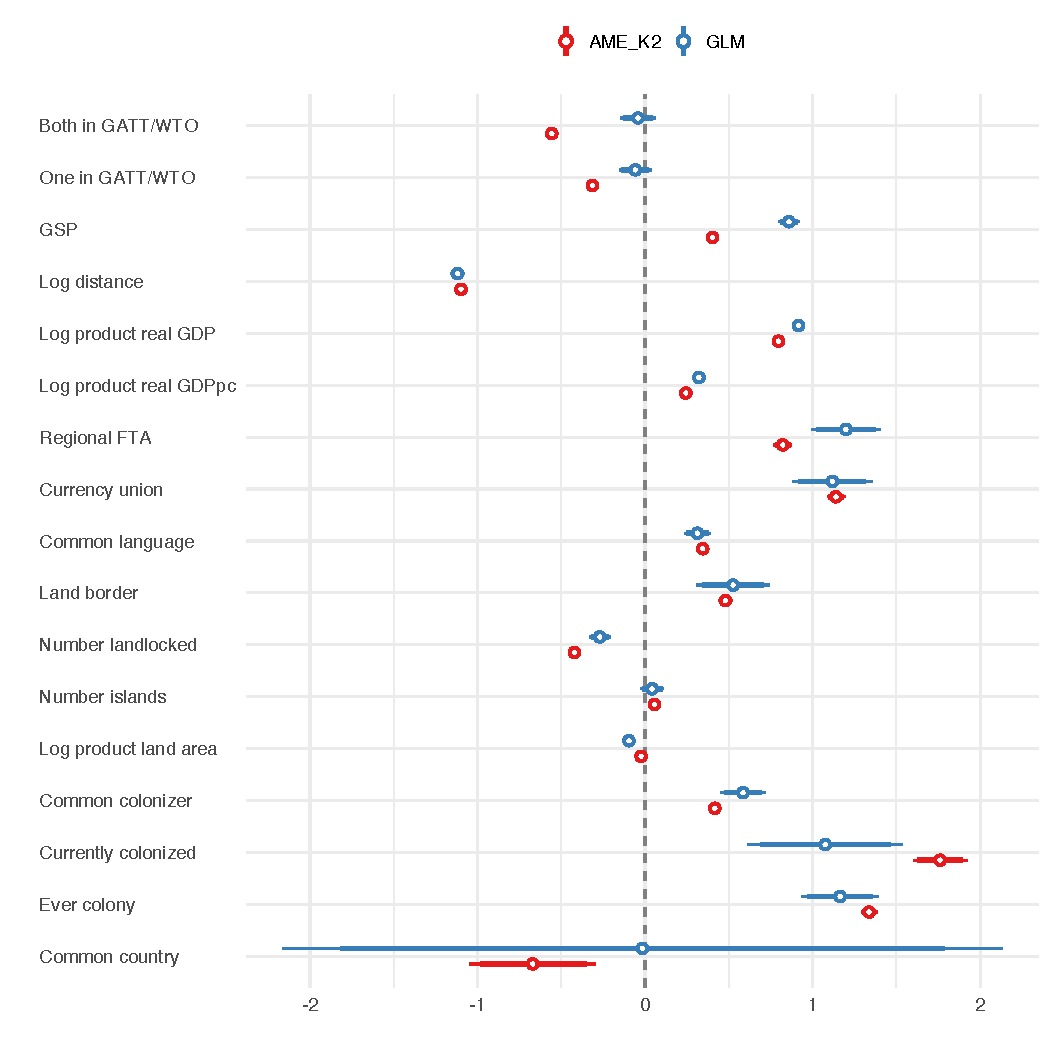
\includegraphics[width=\textwidth]{rose_coefs_all_final.pdf}
% \caption{Coefficient plot of Rose (2004)'s original model (blue) compared to AME model (red).}\label{fig:roseCoef}
%\end{figure}

\begin{figure}
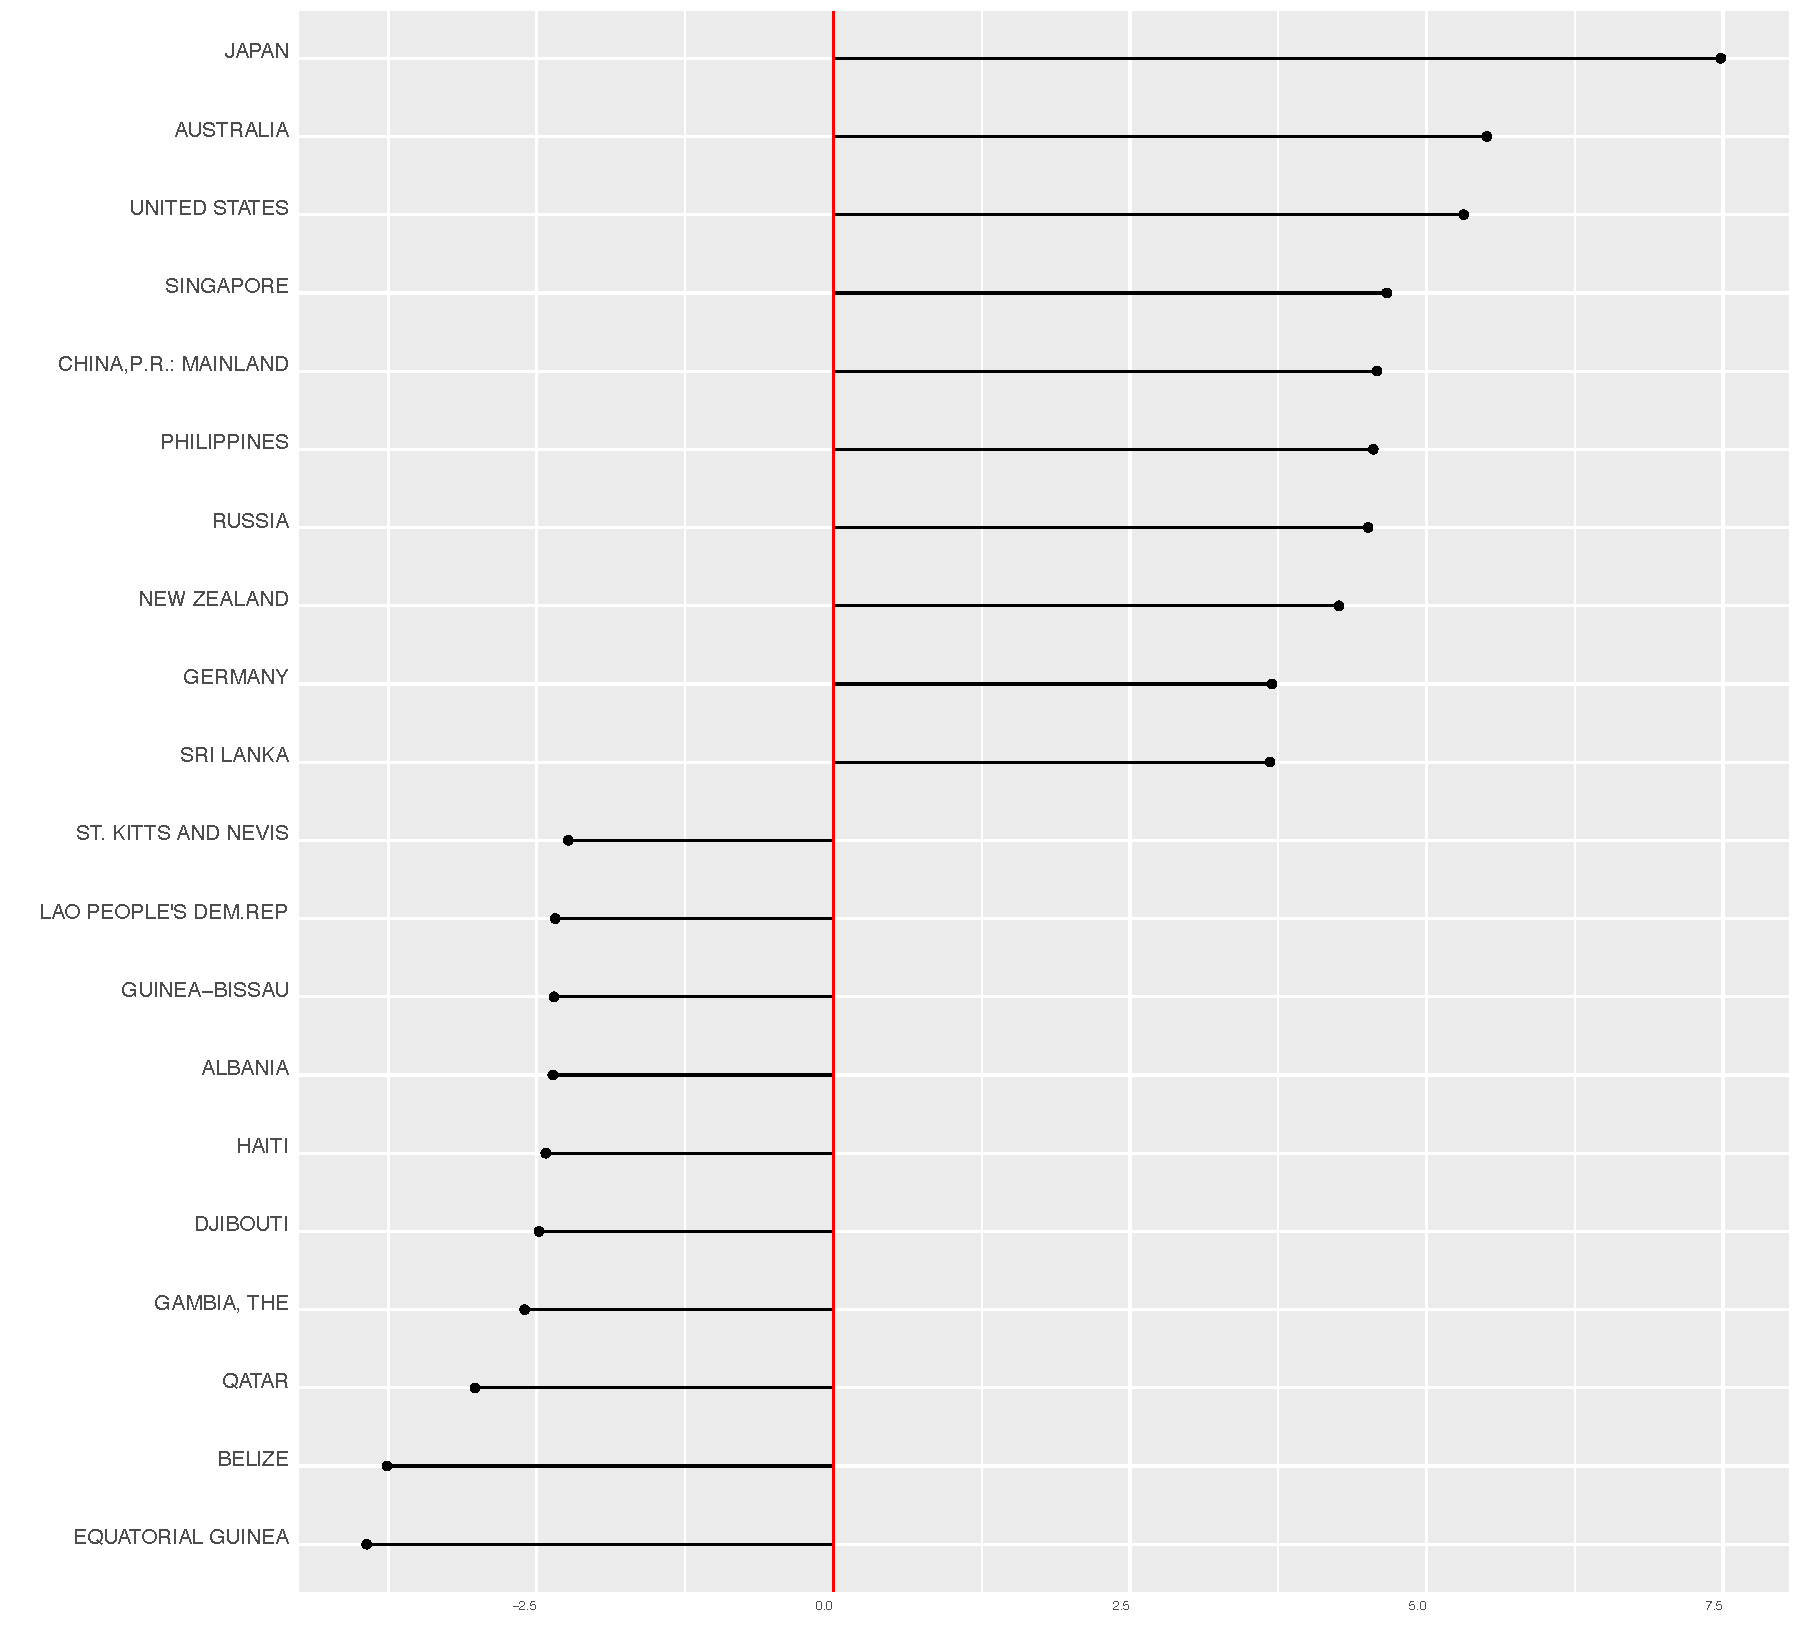
\includegraphics[width=\textwidth]{ABplot_rose_top10.pdf}
 \caption{Nodal Random Effects for AME estimation of Rose (2004).}\label{fig:roser}
\end{figure}

%\begin{figure}
%\centering   
%\subfigure[Nodal Random Effects]%{\label{fig:rosesend}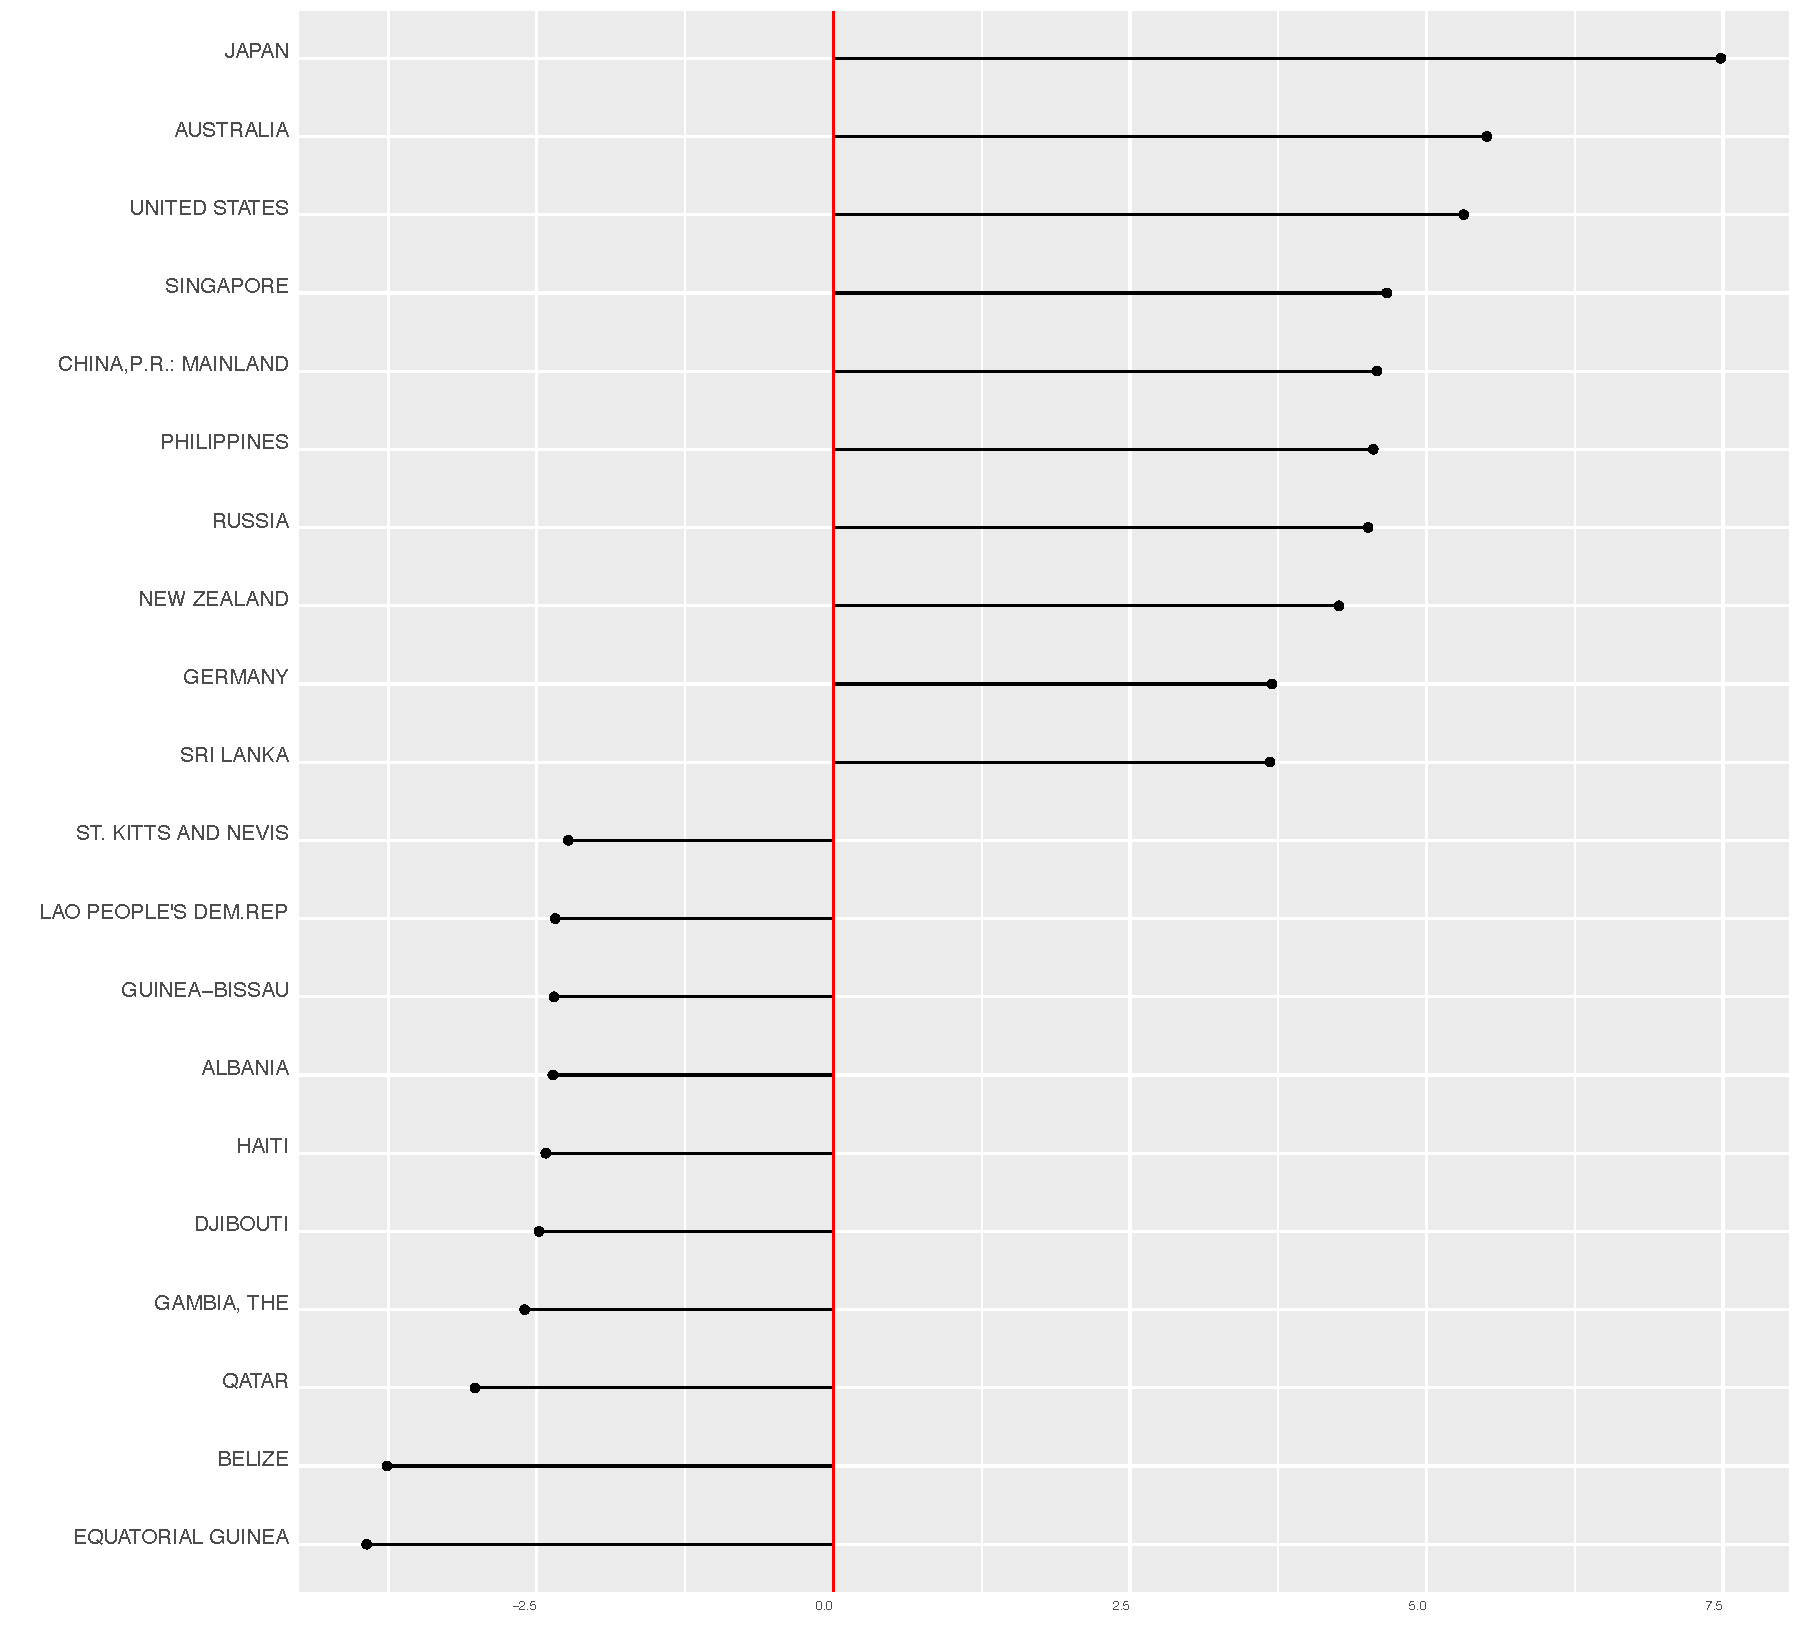
\includegraphics[width=65mm]{ABplot_rose_top10.pdf}}
%\subfigure[Receiver Random Effects]{\label{fig:rosereceive}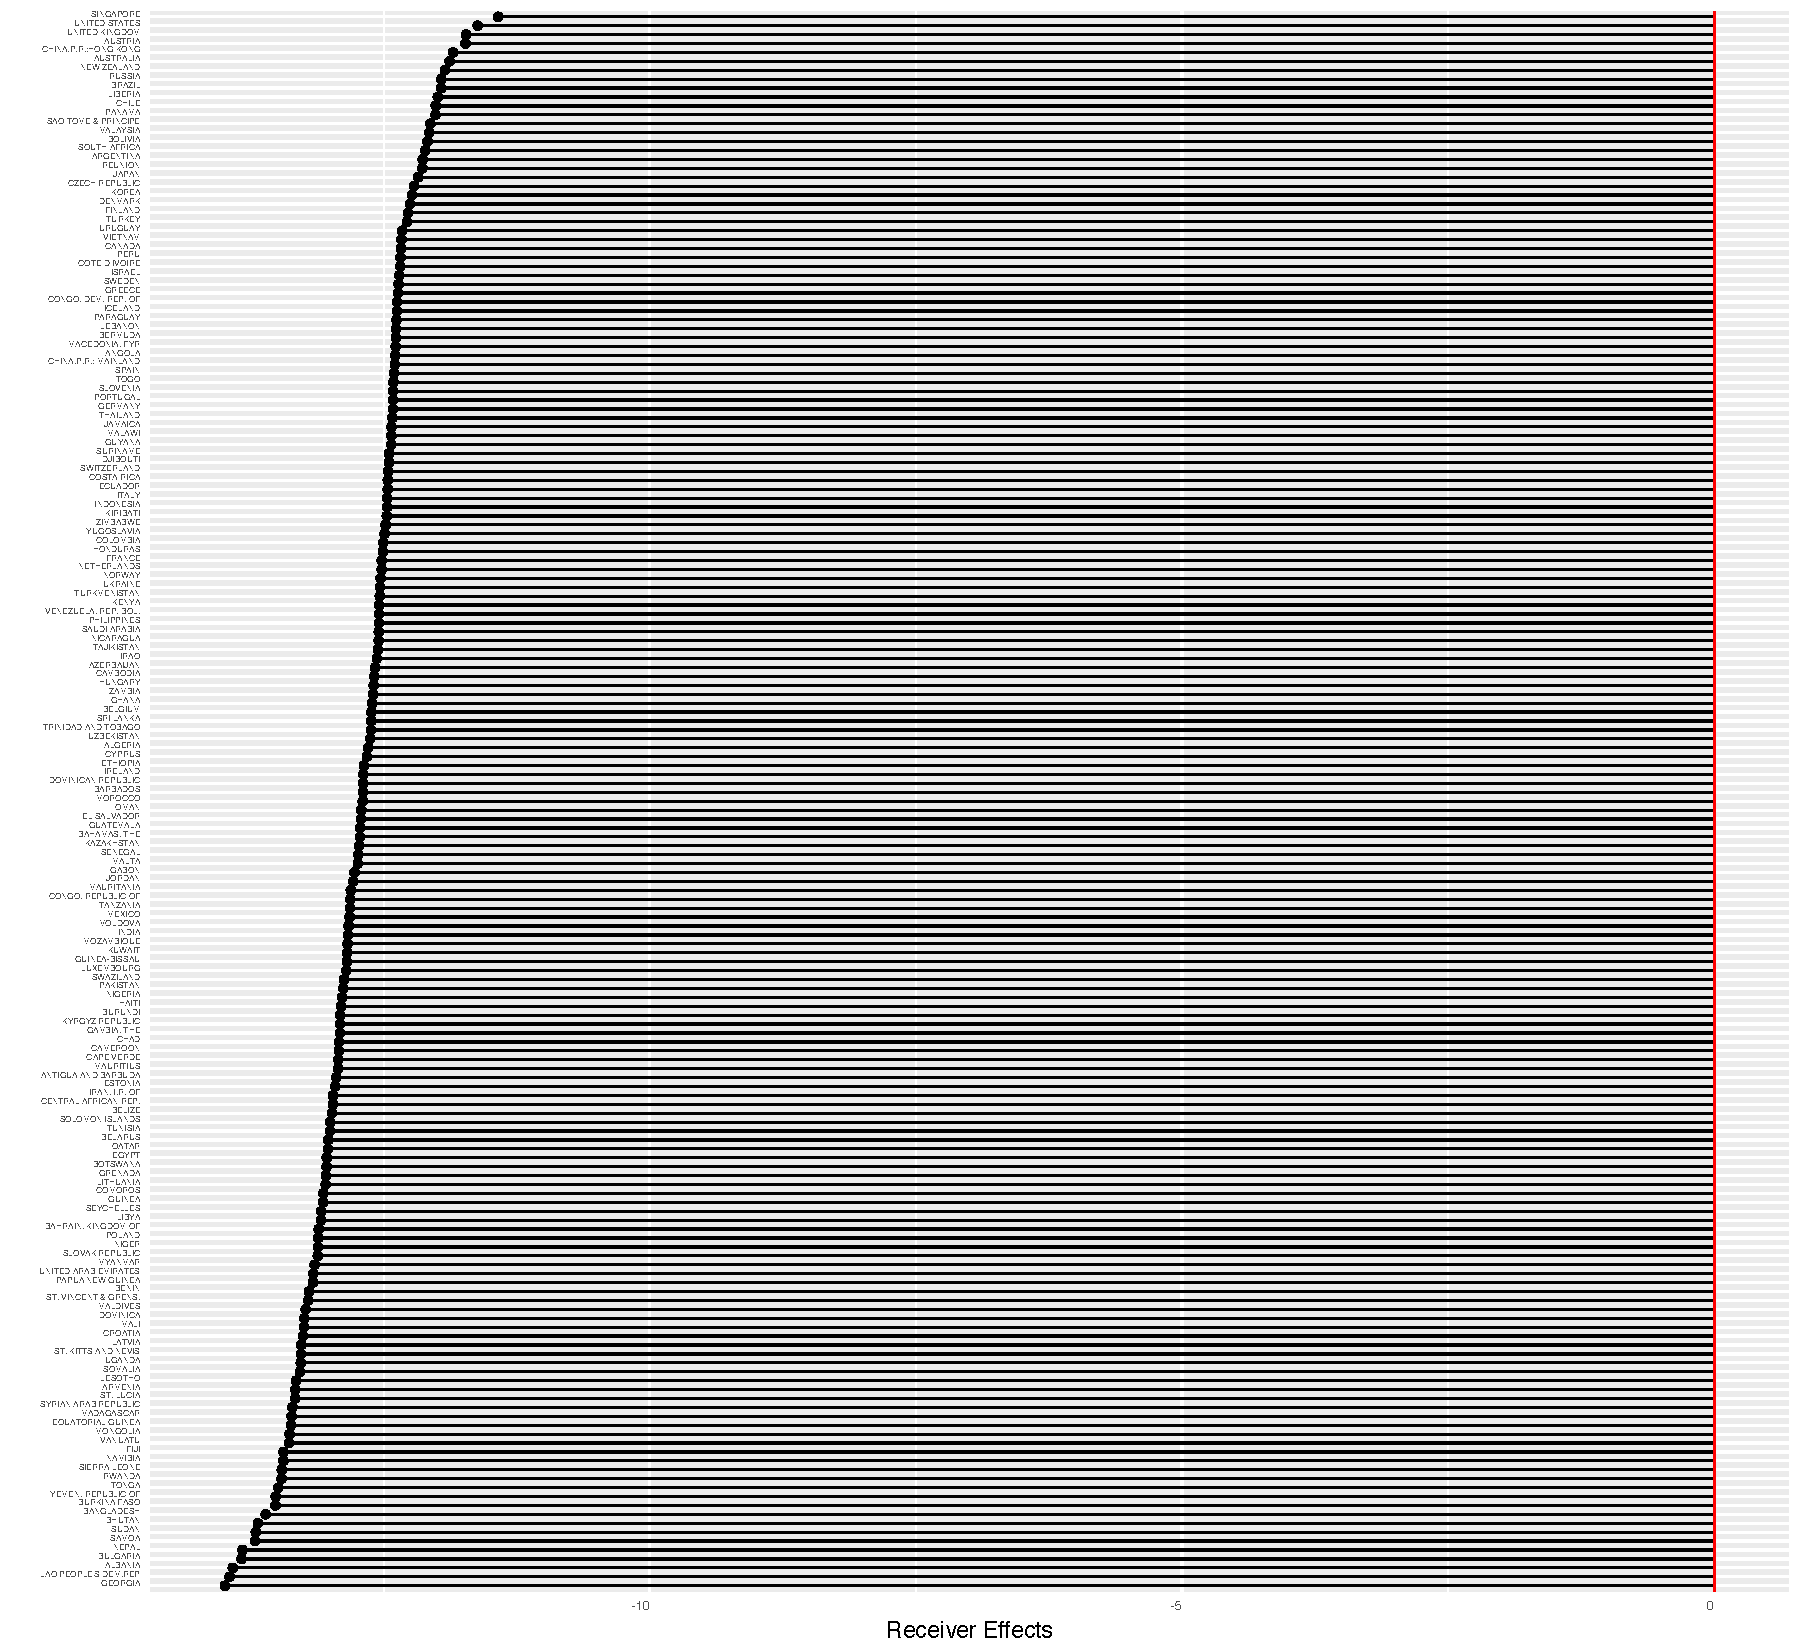
\includegraphics[width=65mm]{ABplot_receiver_rose.pdf}}
%\caption{Sender and receiver random effects for AME estimation of Rose (2004).}
%\label{fig:rosesr}
%\end{figure}

\newpage
\subsection{Replication of McDonald (2004)}

\citet{mcdonald:2004} studies whether trade promotes peace between nations. The link between conflict and trade is perplexing, with many presistent, yet competing explanations. \citet{mcdonald:2004} includes the argument that interdependence between states ``makes conflict less likely because of its efficiency over conquest in acquiring resources\ldots (547)''. Accordingly, his primary contribution is to provide evidence challenging the generalized linkage between peace and trade and to offer a new measurement of the key independent variable, trade. \citet{mcdonald:2004} refines the trade variable, arguing that \textit{free} trade, rather than trade alone, reduces the likelihood of conflict between states. His key hypothesis that greater levels of protection increase the probability of interstate conflict, an argument that builds on the work of classic liberalism and connects free trade to the power of domestic audiences. \citet{mcdonald:2004} measures free trade in two ways. The first captures the idea that larger protected sectors generate greater societal pressures resulting in pockets of support for war. This protection variable measures the proportion of customs revenue divided by total imports in the state that possesses the greater such ratio in each dyad. This measure captures the score of the state in the dyad that possesses higher barriers to trade (560). \citet{mcdonald:2004} also includes a measure of economic integration  calculated as ``the lower proportion of total dyadic trade (imports plus exports) divided by state $i$'s GDP or total dyadic trade divided by state $j$'s GDP'' (560). The binary, dependent variable is the onset of a new militarized interstate dispute within a given dyad. \citet{mcdonald:2004} employs logistic regression to examine the putative statistical significance of these variables. The models include splines to correct for temporal dependence, and robust standard errors clustered on each dyad.

% TO DO: include discussion and analysis of different K's in appendix (for M cD)
\begin{figure}
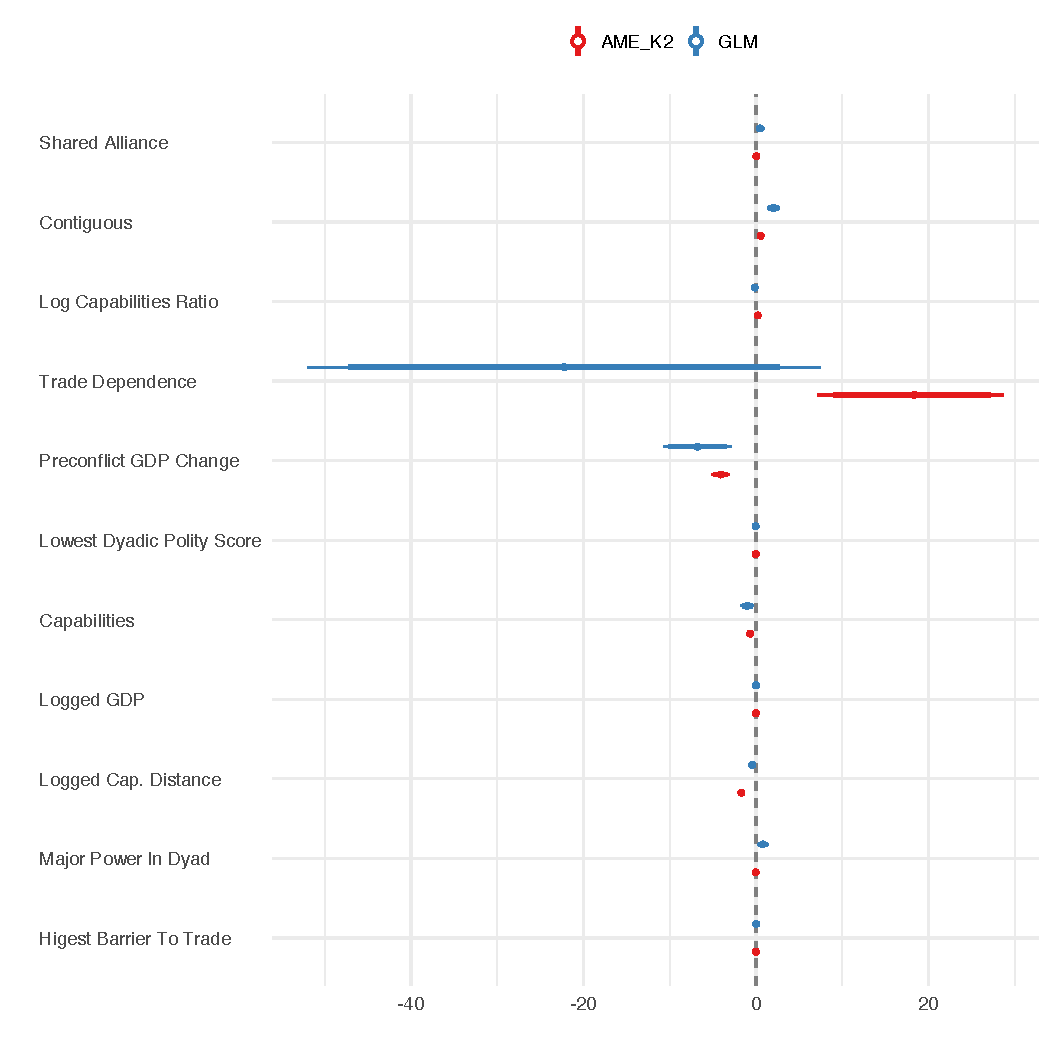
\includegraphics[width=\textwidth]{McDonald_coefs.pdf}
\caption{\label{fig:mcdCoefs}Coefficient plot of McDonald (2004)'s original model (blue) compared to AME model (red).}
\end{figure}

%\begin{figure}
%\centering   
%\subfigure[AUC]{\label{fig:mcDauc}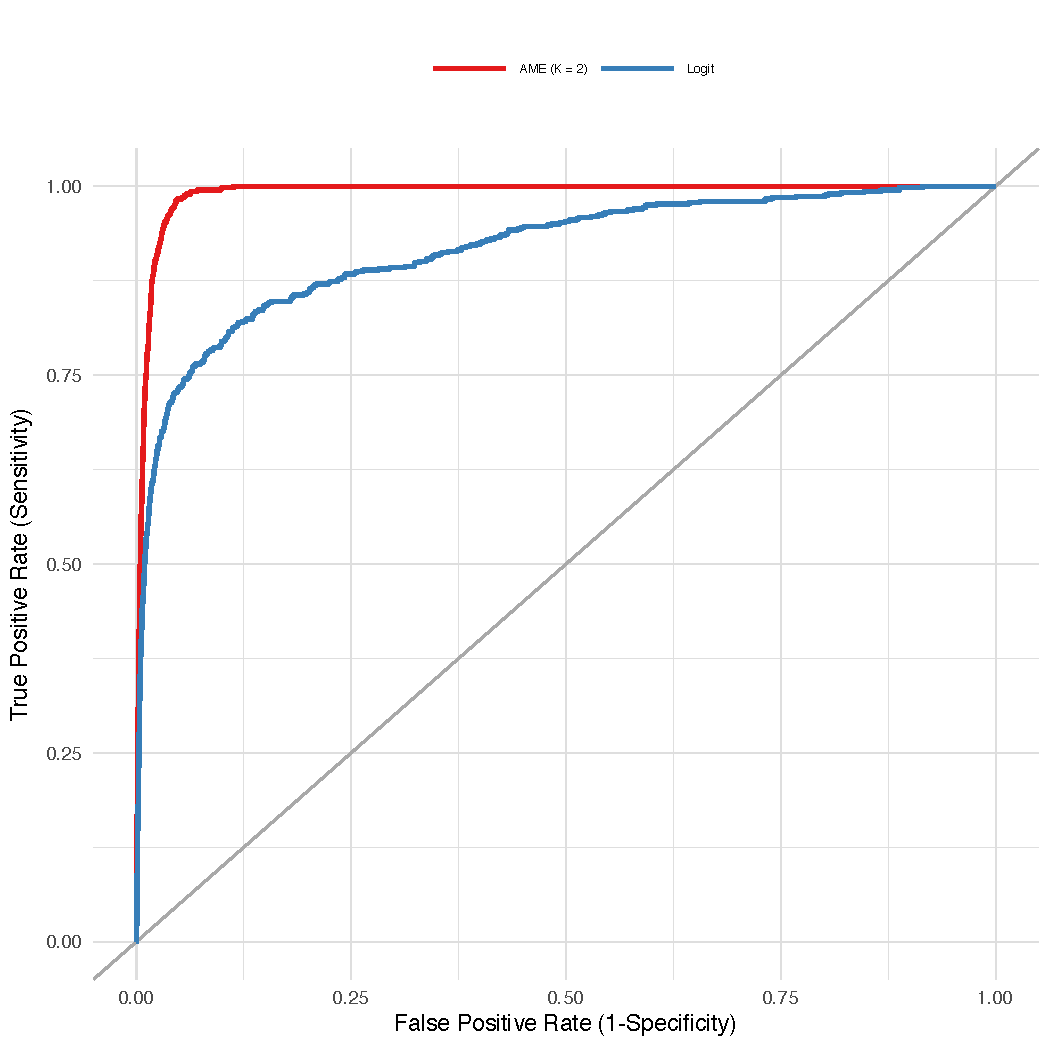
\includegraphics[width=65mm]{McDonald_auc_outsamp.pdf}}
%\subfigure[Precision and Recall]{\label{fig:mcDpr}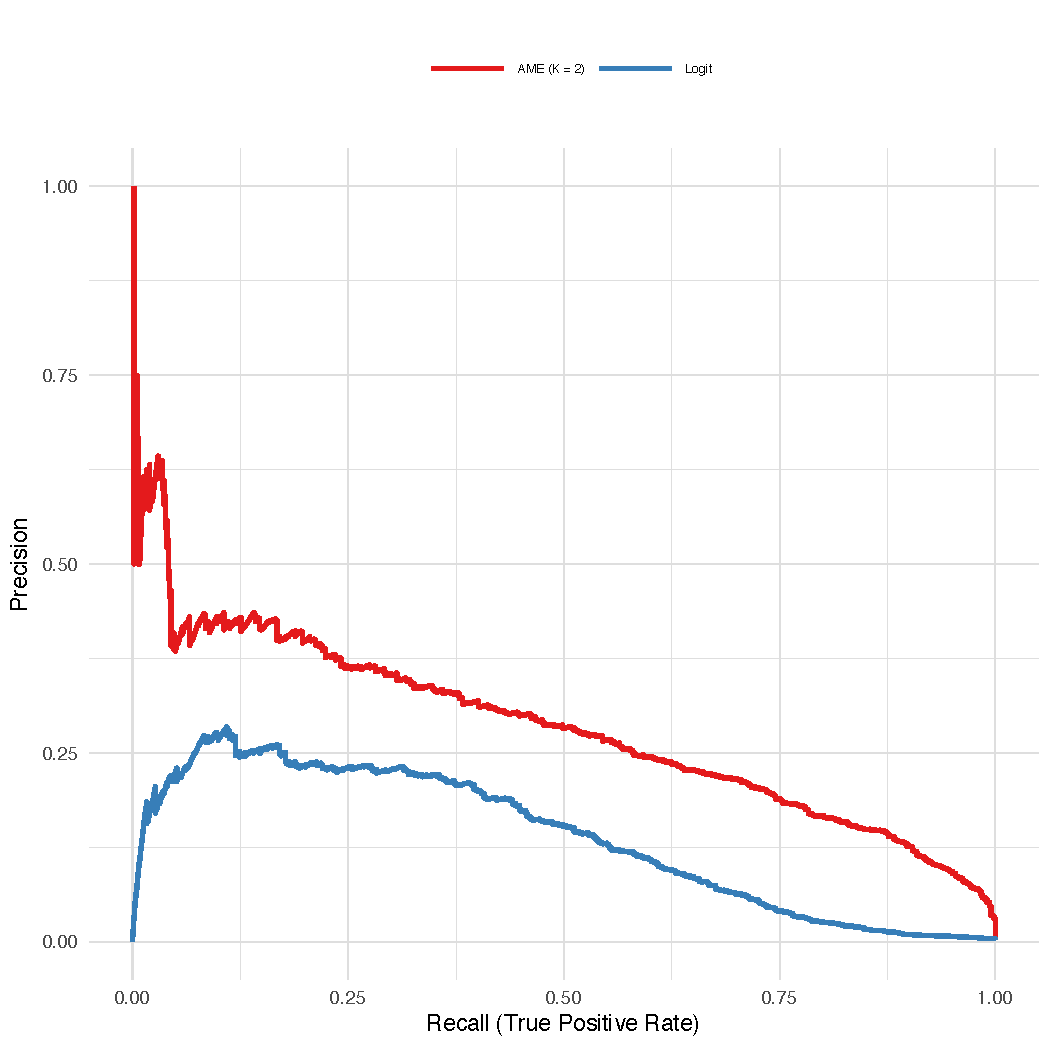
\includegraphics[width=65mm]{McDonald_pr_outsamp.pdf}}
%\caption{\label{fig:mcdall} Assessments of out-of-sample predictive performance for McDonald (2004) using ROC curves and PR curves.}
%\end{figure}

% TO DO: fix bib

Our replication reveals that trade relations are highly interdependent and exhibit important patterns of transitivity.  Or, in other words, if countries $i$ and $j$ are highly dependent and countries $j$ and $k$ are also highly dependent, then we are likely to observe high dependency between countries $i$ and $k$. Our findings support those of Traag and Lupu (2013) which argue that indirect trade relations reduce the probability of conflict. This indicates that conflict is less likely between members of a trade community. Once we control for these dependencies, we can more clearly interpret the positive link between trade and conflict. Figure~\ref{fig:mcdCoefs} shows the coefficients for both the original and AME model. The most striking thing is that AME finds a positive---not negative as found by McDonald---association between trade dependence and conflict. The AME coefficient is not only in the opposite direction, but it is approximately three times more precisely estimated.  At the same time, the AME has ROC and PR curves (not shown) that dominate the OLS results found in McDonald (2004).



\subsection{Replication of Gibler (2017)}

% We chose this article because it is published in 2017, demonstrating that the concern with interdependence continues to the present and because it was published in the so-called flagship journal of political science, \textit{The American Political Science Review.} It examines the link between dyadic capability differences and international conflict in terms of how and when states became independent members of the international system.  It assumes that membership in the international system---defined in typical ways---has a substantial influence on capabilities. In the same way that capabilities don't seem to vary enormously over time, at least comparatively, states become independent in a particular location, clustered with surrounding states. Neither does this change much over time. Gibler shows that the long-standing relationship between the relative parity of capabilities and initiation of international conflict is almost completely mediated by the initial conditions for the members of the dyad when they joined the international system as sovereign members. This finding calls into question many IR theories about the role of balance in terms of generating international conflict \citep{organski:1958}.

The replications we have undertaken are all from articles over the past fifteen years.  A more recent example is \citet{gibler:2017} which examines the onset of militarized disputes using capabilities, joint democracy, alliances, and power parity in a undirected dyadic study using logistic regression and dyad clustered standard errors.   In addition to this, Gibler shows that the long-standing relationship between the relative parity of capabilities and initiation of international conflict is almost completely mediated by the initial conditions for the members of the dyad when they joined the international system as sovereign members. This finding calls into question many IR theories about the role of balance in terms of generating international conflict \citep{organski:1958}.

\begin{table}
\begin{center}
\caption{Comparison of Gibler (2017) Model 6 results with AME results. This was run over a chain of $10,000$ iterations.  \label{tab:gibme}}
\begin{tabular}{lrr} \toprule
& \multicolumn{2}{c}{$\hat{\beta}$ Estimates}\\ \cmidrule{2-3}
Variable & \texttt{logit} & \texttt{amen} \\ \midrule
Allied & 0.142&  0.023 \\
Joint Democracy &\bf -0.507&  0.045 \\
Peace Years \bf &-0.260& \bf -0.060 \\
Spline 1 &\bf -0.001& \bf 0.00 \\
Spline 2&\bf -0.000& \bf 0.00\\
Spline 3 &-0.000& \bf 0.00\\ 
Contiguity &\bf 2.412& \bf 0.640 \\
Parity &0.075&  -0.013 \\
Parity at entry year&\bf 0.868&  0.002 \\ 
Rivalry &\bf 2.031&\bf 0.721\\ 
Constant &\bf -5.526 & \bf  -2.581\\ \bottomrule
\end{tabular}\\
\end{center}
{\bf Note}: {\bf Bold} indicates conventional statistical significance at $p < 0.05$ or less in Gibler (2017). For comparative purposes, only, we have employed the same criterion to the results from the \texttt{amen} estimation.
\end{table}

We re-estimated model 6 from Table 6 (2017,34). The results are presented in Table~\ref{tab:gibme} in order to facilitate explicit comparison.
The results obtained with \texttt{amen} stand in stark contrast to those found with a logistic regression (with dyad clustered, robust standard errors).  Most importantly, the primary variable from the Gibler study, parity of the members of a dyad at the year in which they entered the international system, is shown to be unimportant in the amen results.  Not only is the value of the this parameter small, but it has a very large relative standard error, over a magnitude larger than the parameter itself ($z= 0.038$). In addition, joint democracy follows the same pattern of importance in the logistic results, but this disappears once interdependencies are modeled.  As might be expected the strong geographic clustering in the original study is about one-quarter as strong in the \texttt{amen} estimations. Similarly, rivalry coefficients are about one-third the size in the \texttt{amen} formulation, but a great deal more precisely measured ($z=18.116$). 

Beyond more informative fixed effect coefficients, the \texttt{amen} approach also provides information about the interdependencies that were modeled. The most pertinent of these may be the dyadic and triadic dependencies which are presented in Figure~\ref{fig:gibler:dyadtriad}, which further reveal that the assumption of independence among the dyadic data in this study can be strongly rejected. Perhaps most importantly, the main substantive conclusions of the 2017 Gibler study do not seem warranted from the perspective of the results obtained with the \texttt{amen} estimation that explicitly models \first- \second-, and \third-order interdependencies. Not only do the estimated coefficients tell a different story, but the assumptions under which the original results would hold are shown to be violated by the data.

% sd.rowmean sd.colmean   dyad.dep  triad.dep 
% 0.03210221 0.03210221 0.99362646 0.00130249 
\begin{figure}
\caption{\label{fig:gibler:dyadtriad} The left panel is  a plot of the dyadic dependencies in the Gibler model 6; the right panel shows the triad dependencies.  Note that the red line represents the null hypothesis of no dependencies, indicating that the standard logistic approach is far from what is uncovered with this analysis. }
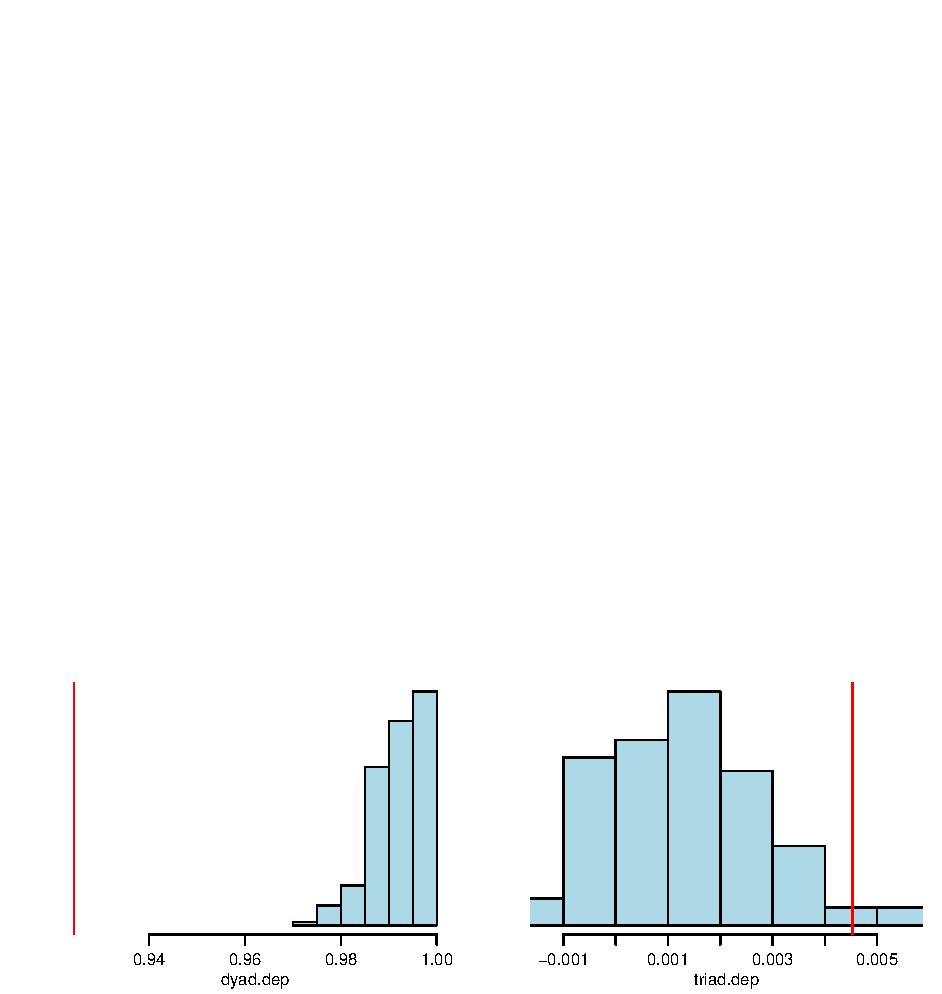
\includegraphics[width=\textwidth]{netplots}
\end{figure}
\FloatBarrier

\section{\textbf{Conclusion}}

International relations is generally about the interactions and dependencies among a set of countries or other important actors such as international governmental organizations (IGOs). This is particularly true of those scholars who work in the tradition of the Correlates of War Project, but is by no means limited to them.\footnote{See \cite{singer:1972} for an early description of the project and also see the project's Web site for an history and more recent efforts \url{http://www.correlatesofwar.org/}.} Many scholars have debated the use and abuse of dyadic data.\footnote{One recent on-line symposium can be found at \url{http://bit.ly/2wB2hab}.} It is clear from a survey of the literature and from work in this area published as recently as 2017 that many find dyadic data to be an important touchstone in the study of international relations \citep{erikson:pinto:2014,aronow:etal:2015}.

At the same time, we know that research designs focusing on the statistical analysis of dyadic data quickly go astray if the dyadic data are assumed to be iid.  Virtually all of the standard statistical models---ordinary least squares and logistic regressions, to name a few---fail if the data are not conditionally independent. This fact has been accepted when it comes to temporal dependencies, but adoption of methods to account for network dependencies have seen less progress. By definition dyadic data are not iid and thus the standard approaches can not be used cavalierly to analyze these data.  \citet{signorino:1999} showed why this is true of models of strategic interaction, but it is more broadly true of models that employ dyadic data.  We show that the AME framework can be employed to account for the statistical issues that arise when studying dyadic data.

% These approaches have been developed for a while, but are not yet widely used in international relations scholarship.  The latent network model captures first-order dependencies (the tendencies of certain actors to send and receive more of a certain action), second-order dependencies (the tendency of actors to reciprocate actions), and third-order dependencies (the ability for actions within a dyad to effect a third party) in dyadic data using a familiar regression framework that has been adapted for relational data---such as dyadic data---which are not independent nor identically distributed.

To explore this approach in the context of international relations we have presented two broad analyses. The first is a simulation where the characteristics of the network are known. This shows that, when there are unobserved dependencies, the AME approach is less biased in terms of parameter estimation compared with standard approach employed in international relations to study dyadic data (i.e., GLM models). The second is a replication of five prominent studies that have been published recently using a broad range of dyadic data to draw inferences about international relations.  These five studies have been replicated with the original research designs, each of which used a statistical method that assumes the dyadic data are all independent from one another.  We then re-analyzed each study using the AME model.  In every case, we found that the AME approach provided a) increased precision of estimation, b) better out-of-sample fits, c) evidence of 1st-, 2nd-, and 3rd-order dependencies that were overlooked in the original studies.\footnote{The Appendix contains performance data on all of these replications, as well as sample code illustrating how to undertake AME analysis using \texttt{amen}.} In several cases, the new approach overturns the basic findings of the original research.  This leads us to speculate that many of the findings in the international relations literature may be fragile in the sense that they can only be obtained under stringent assumptions that cannot possibly be valid.  In turn, this leads to a certain arbitrariness in some research findings, which might lead to puzzles that are more apparent than real \citep{zinnes:1980}.  

It is no longer necessary to assume that the interesting, innate interdependencies in relational data about international relations can be ignored. Nor do they have to be approximated with \textit{ad hoc}, incomplete solutions that purport to control for dependencies (such as modifying the post-estimation standard errors of the estimated coefficients \citep{king:roberts:2014}). Instead, the interdependencies may be addressed directly with additive and multiplicative effects in the context of a generalized linear model that provides more reliable inferences, better out-of-sample predictive performance, and new substantive insights. 

% We also examine each of the models using the AME framework described above.  Our goal is to ascertain whether accounting for the statistical complications that arise in dyadic data result in different model estimates when addressed in an AME framework, and more importantly we highlight the substantive opportunities presented by our alternative approach.

% Based in part on our results as well as the statistical characteristics of the AME framework, we believe that it does. The dynamic latent factor model provides a step forward in the modeling of international relations.

\newpage
% Bib stuff
\clearpage

% \bibliography{C:/Users/Owner/whistle/master}
\bibliography{C:/Users/herme/whistle/master}
%\bibliography{/Users/maxgallop/documents/whistle/master}
%\bibliography{/Users/s7m/whistle/master}
% \bibliography{/Users/mdw/Git/whistle/master}
 % \bibliography{/Users/dorffc/ProjectsGit/whistle/master}
% \bibliographystyle{authordate1}
\bibliographystyle{sm}
% \clearpage
% \section*{All About Us}

\appendix
\clearpage

\renewcommand{\thefigure}{A\arabic{figure}}
\setcounter{figure}{0}
\renewcommand{\thetable}{A.\arabic{table}}
\setcounter{table}{0}
\renewcommand{\thesection}{A.\arabic{section}}
\setcounter{section}{0}

\section*{\textbf{Appendix}}

\subsection*{Additional Replication Information}

\subsubsection*{Gibler (2017)}

Coefficient plot and performance comparison.

% latex table generated in R 3.4.1 by xtable 1.8-2 package
% Sat Oct 21 23:10:24 2017
\begin{table}[ht]
\centering
\begingroup\normalsize
\begin{tabular}{lccc}
 Variable & GLM (Logit) & GLM (Probit) & AME \\ 
  \hline
\hline
(Intercept) & $-5.826$ & $-2.793$ & $-2.758$ \\
   & (0.366) & (0.366) & (0.045) \\ 
  Allied & 0.133 & 0.067 & $0.078$ \\
   & (0.102) & (0.102) & (0.021) \\ 
  Joint Democracy & $-0.527$ & $-0.186$ & 0.005 \\
   & (0.099) & (0.099) & (0.022) \\ 
  Peace Years & $-0.261$ & $-0.099$ & $-0.058$ \\
   & (0.016) & (0.016) & (0.004) \\ 
  Spline 1 & $-0.001$ & $0.000$ & $0.000$ \\
   & (0.000) & (0.000) & (0.000) \\ 
  Spline 2 & $0.000$ & $0.000$ & $0.000$ \\
   & (0.000) & (0.000) & (0.000) \\ 
  Spline 3 & 0.000 & 0.000 & $0.000$ \\
   & (0.000) & (0.000) & (0.000) \\ 
  Contiguity & $2.427$ & $0.95$ & $0.66$ \\
   & (0.196) & (0.196) & (0.023) \\ 
  Parity & -0.77 & -0.228 & -0.067 \\ 
   & (0.551) & (0.551) & (0.057) \\ 
  Parity at Entry Year & $2.034$ & 0.739 & -0.05 \\
   & (0.617) & (0.617) & (0.065) \\ 
  Rivalry & $2.034$ & $1.035$ & $0.655$ \\
   & (0.213) & (0.213) & (0.028) \\ 
   \hline
\hline
\end{tabular}
\endgroup
\caption{Parameter comparison for Gibler (2017). Standard errors in parentheses.} 
\label{tab:gibler_coef}
\end{table}

\FloatBarrier

\begin{figure}
	\centering   
	\subfigure[AUC]{\label{fig:giblerroc}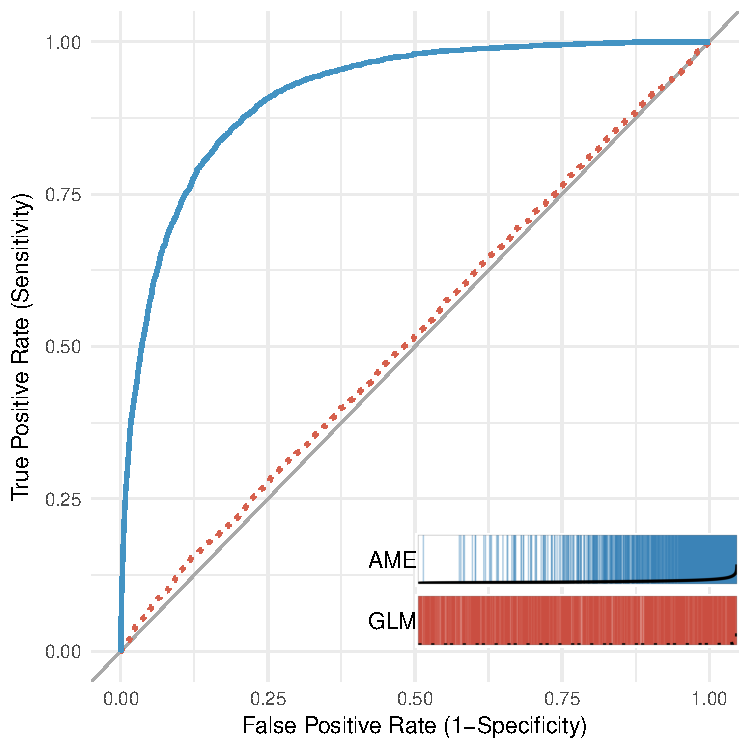
\includegraphics[width=.45\textwidth]{gibler_roc_outSample.pdf}}
	\subfigure[Precision and Recall]{\label{fig:giblerpr}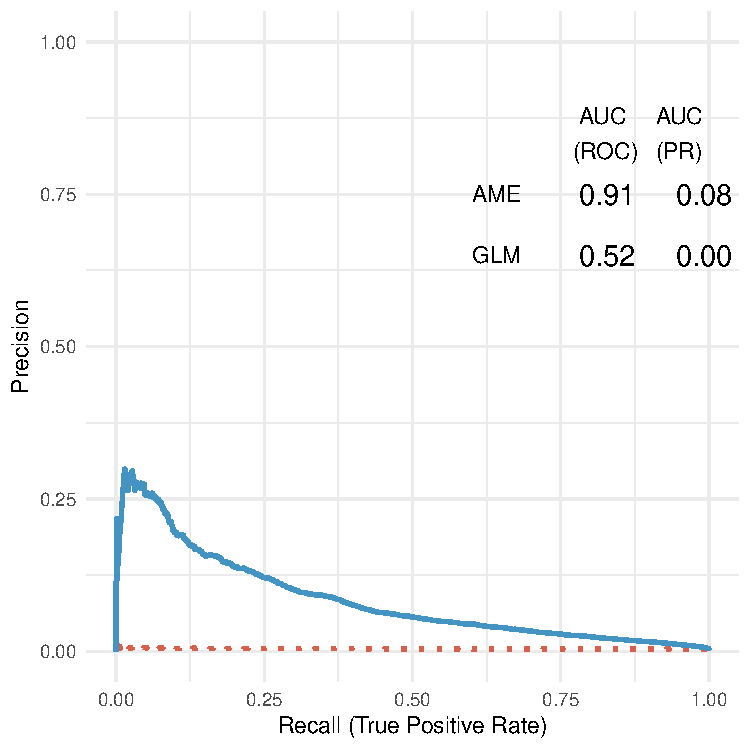
\includegraphics[width=.45\textwidth]{gibler_pr_outSample.pdf}}
	\caption{Assessments of out-of-sample predictive performance for Gibler (2017) using ROC curves and PR curves.}
\end{figure}
\FloatBarrier

\clearpage
\subsubsection*{McDonald (2004)}

Coefficient plot and performance comparison.

% latex table generated in R 3.4.1 by xtable 1.8-2 package
% Sat Oct 21 23:10:32 2017
\begin{table}[ht]
\centering
\begingroup\normalsize
\begin{tabular}{lccc}
 Variable & GLM (Logit) & GLM (Probit) & AME \\ 
  \hline
\hline
(Intercept) & 0.054 & 0.085 & $-1.171^{\ast\ast}$ \\ 
   & (1.179) & (0.409) & (0.096) \\ 
  Spline0 & $-0.438^{\ast\ast}$ & $-0.222^{\ast\ast}$ & $-0.145^{\ast\ast}$ \\ 
   & (0.061) & (0.026) & (0.019) \\ 
  Spline1 & $-0.003^{\ast\ast}$ & $-0.002^{\ast\ast}$ & $-0.001^{\ast\ast}$ \\ 
   & (0.001) & (0.000) & (0.000) \\ 
  Spline2 & 0.001 & $0.001^{\ast\ast}$ & $0.000^{\ast}$ \\ 
   & (0.001) & (0.000) & (0.000) \\ 
  Spline3 & 0.000 & 0.000 & $0.000^{\ast\ast}$ \\ 
   & (0.000) & (0.000) & (0.000) \\ 
  Shared Alliance & $0.483^{\ast\ast}$ & 0.155 & $0.342^{\ast\ast}$ \\ 
   & (0.233) & (0.095) & (0.069) \\ 
  Contiguous & $2.011^{\ast\ast}$ & $0.789^{\ast\ast}$ & $0.988^{\ast\ast}$ \\ 
   & (0.343) & (0.118) & (0.066) \\ 
  Log Capabilities Ratio & $-0.146^{\ast\ast}$ & $-0.054^{\ast\ast}$ & $0.029^{\ast\ast}$ \\ 
   & (0.072) & (0.026) & (0.013) \\ 
  Trade Dependence & -22.244 & -7.051 & $-13.134^{\ast\ast}$ \\ 
   & (15.184) & (5.536) & (4.938) \\ 
  Preconflict GDP Change & $-6.79^{\ast\ast}$ & $-3.155^{\ast\ast}$ & $-2.651^{\ast\ast}$ \\ 
   & (2.033) & (0.788) & (0.574) \\ 
  Lowest Dyadic Polity Score & $-0.036^{\ast\ast}$ & $-0.014^{\ast\ast}$ & $-0.026^{\ast\ast}$ \\ 
   & (0.015) & (0.006) & (0.002) \\ 
  Capabilities & $-0.995^{\ast\ast}$ & $-0.349^{\ast\ast}$ & 0.022 \\ 
   & (0.377) & (0.14) & (0.079) \\ 
  Logged GDP & $0.000^{\ast\ast}$ & $0.000^{\ast\ast}$ & $0.000^{\ast\ast}$ \\ 
   & (0.000) & (0.000) & (0.000) \\ 
  Logged Cap. Distance & $-0.425^{\ast\ast}$ & $-0.224^{\ast\ast}$ & $-0.275^{\ast\ast}$ \\ 
   & (0.14) & (0.047) & (0.012) \\ 
  Major Power In Dyad & $0.769^{\ast\ast}$ & $0.312^{\ast\ast}$ & $0.212^{\ast\ast}$ \\ 
   & (0.322) & (0.122) & (0.098) \\ 
  Higest Barrier To Trade & $0.024^{\ast\ast}$ & $0.011^{\ast\ast}$ & $0.004^{\ast\ast}$ \\ 
   & (0.008) & (0.003) & (0.001) \\ 
   \hline
\hline
\end{tabular}
\endgroup
\caption{Parameter comparison for McDonald (2004). Standard errors in parentheses. $^{**}$ and $^{*}$ indicate significance at $p<0.05$ and $p<0.10$, respectively.} 
\label{tab:mcdonald_coef}
\end{table}

\FloatBarrier

\begin{figure}
	\centering   
	\subfigure[AUC]{\label{fig:mcdonaldroc}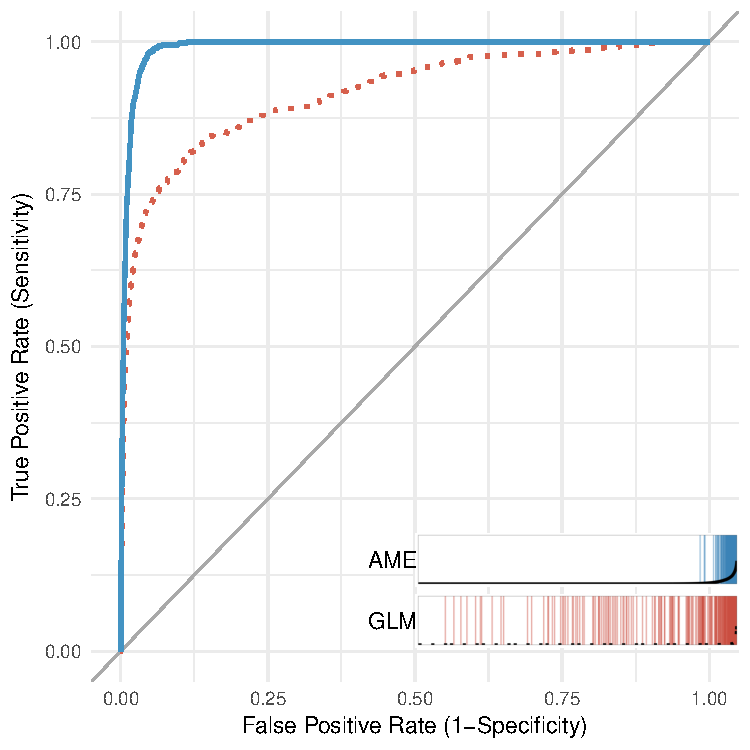
\includegraphics[width=.45\textwidth]{mcdonald_roc_outSample.pdf}}
	\subfigure[Precision and Recall]{\label{fig:mcdonaldpr}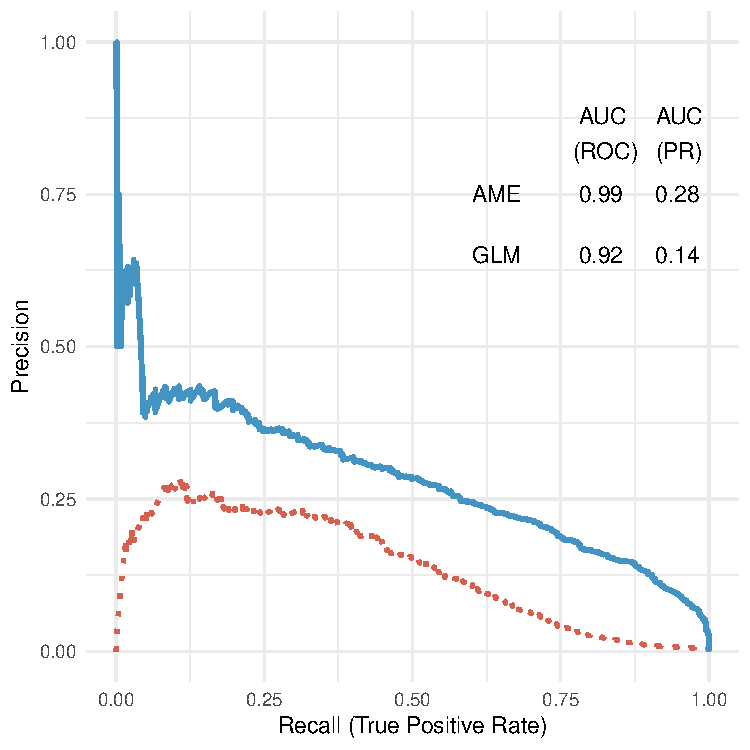
\includegraphics[width=.45\textwidth]{mcdonald_pr_outSample.pdf}}
	\caption{Assessments of out-of-sample predictive performance for McDonald (2004) using ROC curves and PR curves.}
\end{figure}
\FloatBarrier

\clearpage
\subsubsection*{Reiter \& Stam (2003)}

Coefficient plot and performance comparison.

% latex table generated in R 3.4.1 by xtable 1.8-2 package
% Sat Oct 21 23:16:42 2017
\begin{table}[ht]
\centering
\begingroup\normalsize
\begin{tabular}{lccc}
 Variable & GLM (Logit) & GLM (Probit) & AME \\ 
  \hline
\hline
Intercept & $-4.784^{\ast\ast}$ & $-2.339^{\ast\ast}$ & $-3.144^{\ast\ast}$ \\ 
   & (0.097) & (0.034) & (0.06) \\ 
  Pers/Democ Directed Dyad & $1.026^{\ast\ast}$ & $0.378^{\ast\ast}$ & $0.255^{\ast\ast}$ \\ 
   & (0.14) & (0.051) & (0.068) \\ 
  Democ/Pers Directed Dyad & 0.083 & 0.033 & 0.112 \\ 
   & (0.191) & (0.066) & (0.079) \\ 
  Personal & 0.281 & 0.15 & $0.211^{\ast}$ \\ 
   & (0.265) & (0.099) & (0.11) \\ 
  Military & -0.323 & -0.105 & -0.025 \\ 
   & (0.574) & (0.204) & (0.249) \\ 
  Single & $-0.677^{\ast\ast}$ & $-0.261^{\ast\ast}$ & -0.07 \\ 
   & (0.144) & (0.062) & (0.073) \\ 
  Democracy & $-1.073^{\ast\ast}$ & $-0.428^{\ast\ast}$ & $-0.254^{\ast\ast}$ \\ 
   & (0.194) & (0.07) & (0.063) \\ 
  Contiguous & $2.912^{\ast\ast}$ & $1.147^{\ast\ast}$ & $1.296^{\ast\ast}$ \\ 
   & (0.09) & (0.031) & (0.033) \\ 
  Major Power & $2.174^{\ast\ast}$ & $0.919^{\ast\ast}$ & $0.906^{\ast\ast}$ \\ 
   & (0.101) & (0.037) & (0.093) \\ 
  Ally & 0.078 & -0.003 & $0.136^{\ast\ast}$ \\ 
   & (0.086) & (0.035) & (0.037) \\ 
  Higher/Lower Power Ratio & $-0.316^{\ast\ast}$ & $-0.122^{\ast\ast}$ & $-0.111^{\ast\ast}$ \\ 
   & (0.027) & (0.01) & (0.011) \\ 
  Economically Advanced & -0.175 & -0.054 & 0.053 \\ 
   & (0.131) & (0.051) & (0.05) \\ 
  Years Since Last Dispute & $-0.381^{\ast\ast}$ & $-0.149^{\ast\ast}$ & $-0.129^{\ast\ast}$ \\ 
   & (0.023) & (0.009) & (0.008) \\ 
  Cubic Spline 1 & $-0.004^{\ast\ast}$ & $-0.001^{\ast\ast}$ & $-0.001^{\ast\ast}$ \\ 
   & (0.000) & (0.000) & (0.000) \\ 
  Cubic Spline 2 & $0.002^{\ast\ast}$ & $0.001^{\ast\ast}$ & $0.001^{\ast\ast}$ \\ 
   & (0.000) & (0.000) & (0.000) \\ 
  Cubic Spline 3 & $-0.001^{\ast\ast}$ & $0.000^{\ast\ast}$ & $0.000^{\ast\ast}$ \\ 
   & (0.000) & (0.000) & (0.000) \\ 
   \hline
\hline
\end{tabular}
\endgroup
\caption{Parameter comparison for Reiter \& Stam (2003). Standard errors in parentheses. $^{**}$ and $^{*}$ indicate significance at $p<0.05$ and $p<0.10$, respectively.} 
\label{tab:reiter_stam_coef}
\end{table}
\FloatBarrier

\begin{figure}
	\centering   
	\subfigure[AUC]{\label{fig:reiterstamroc}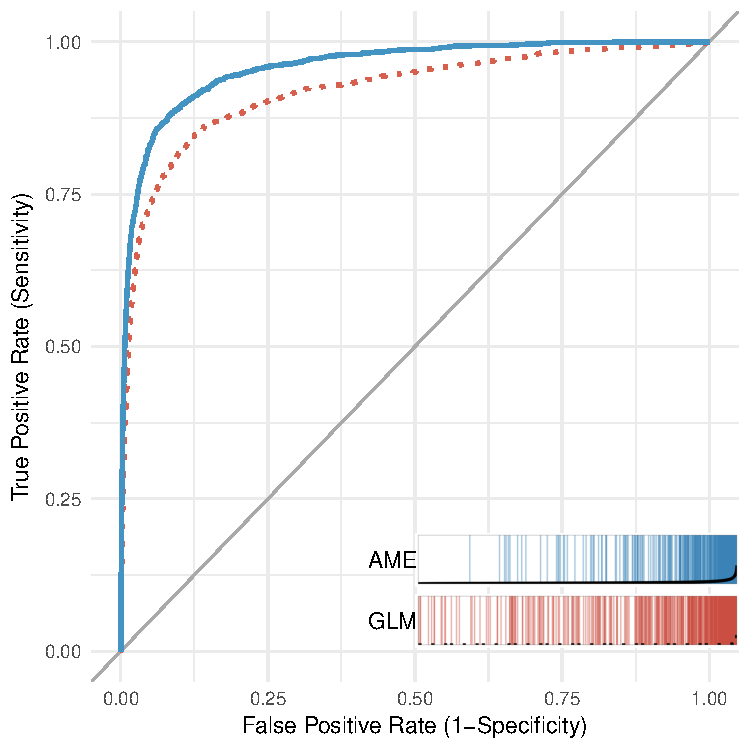
\includegraphics[width=.45\textwidth]{reiter_stam_roc_outSample.pdf}}
	\subfigure[Precision and Recall]{\label{fig:reiterstampr}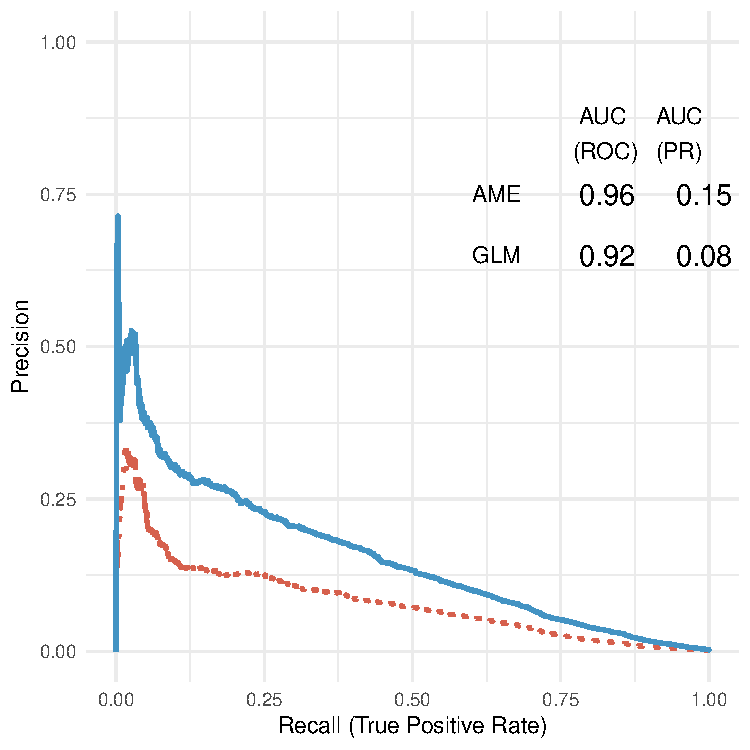
\includegraphics[width=.45\textwidth]{reiter_stam_pr_outSample.pdf}}
	\caption{Assessments of out-of-sample predictive performance for Reiter \& Stam (2003) using ROC curves and PR curves.}
\end{figure}
\FloatBarrier

\clearpage
\subsubsection*{Rose (2004)}

Coefficient plot and performance comparison.

% latex table generated in R 3.4.1 by xtable 1.8-2 package
% Sat Oct 21 22:58:31 2017
\begin{table}[ht]
\centering
\begingroup\normalsize
\begin{tabular}{lcc}
 Variable & LM & AME \\ 
  \hline
\hline
Intercept & $-24.96^{\ast\ast}$ & $-22.532^{\ast\ast}$ \\ 
   & (0.409) & (0.103) \\ 
  Both in GATT/WTO & -0.042 & $-0.56^{\ast\ast}$ \\ 
   & (0.053) & (0.013) \\ 
  One in GATT/WTO & -0.058 & $-0.317^{\ast\ast}$ \\ 
   & (0.049) & (0.012) \\ 
  GSP & $0.859^{\ast\ast}$ & $0.399^{\ast\ast}$ \\ 
   & (0.032) & (0.009) \\ 
  Log Distance & $-1.119^{\ast\ast}$ & $-1.097^{\ast\ast}$ \\ 
   & (0.022) & (0.005) \\ 
  Log Product Real GDP & $0.916^{\ast\ast}$ & $0.798^{\ast\ast}$ \\ 
   & (0.01) & (0.002) \\ 
  Log Product Real GDPpc & $0.321^{\ast\ast}$ & $0.244^{\ast\ast}$ \\ 
   & (0.014) & (0.004) \\ 
  Regional FTA & $1.199^{\ast\ast}$ & $0.826^{\ast\ast}$ \\ 
   & (0.106) & (0.027) \\ 
  Currency Union & $1.118^{\ast\ast}$ & $1.144^{\ast\ast}$ \\ 
   & (0.122) & (0.029) \\ 
  Common language & $0.313^{\ast\ast}$ & $0.345^{\ast\ast}$ \\ 
   & (0.04) & (0.009) \\ 
  Land Border & $0.526^{\ast\ast}$ & $0.483^{\ast\ast}$ \\ 
   & (0.111) & (0.02) \\ 
  Number Landlocked & $-0.271^{\ast\ast}$ & $-0.42^{\ast\ast}$ \\ 
   & (0.031) & (0.009) \\ 
  Number Islands & 0.042 & $0.058^{\ast\ast}$ \\ 
   & (0.036) & (0.009) \\ 
  Log Product Land Area & $-0.097^{\ast\ast}$ & $-0.024^{\ast\ast}$ \\ 
   & (0.008) & (0.002) \\ 
  Common Colonizer & $0.585^{\ast\ast}$ & $0.418^{\ast\ast}$ \\ 
   & (0.067) & (0.013) \\ 
  Currently Colonized & $1.075^{\ast\ast}$ & $1.762^{\ast\ast}$ \\ 
   & (0.235) & (0.081) \\ 
  Ever Colony & $1.164^{\ast\ast}$ & $1.335^{\ast\ast}$ \\ 
   & (0.117) & (0.024) \\ 
  Common Country & -0.016 & $-0.672^{\ast\ast}$ \\ 
   & (1.097) & (0.19) \\ 
   \hline
\hline
\end{tabular}
\endgroup
\caption{Parameter comparison for Rose (2004). Standard errors in parentheses. $^{**}$ and $^{*}$ indicate significance at $p<0.05$ and $p<0.10$, respectively.} 
\label{tab:rose_coef}
\end{table}

\FloatBarrier

% \begin{figure}
% 	\centering   
% 	\subfigure[AUC]{\label{fig:reitaucpr}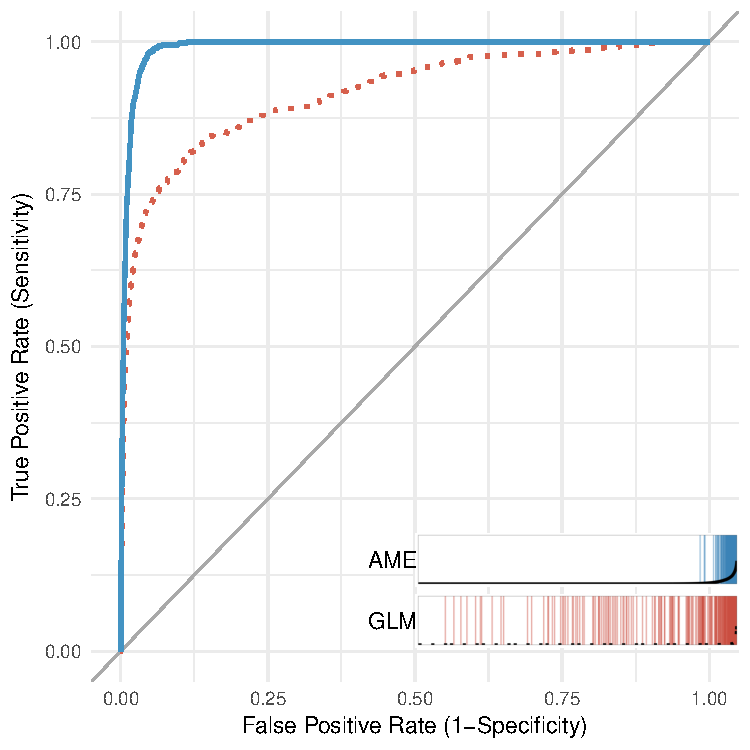
\includegraphics[width=.45\textwidth]{mcdonald_roc_outSample.pdf}}
% 	\subfigure[Precision and Recall]{\label{fig:reitpr}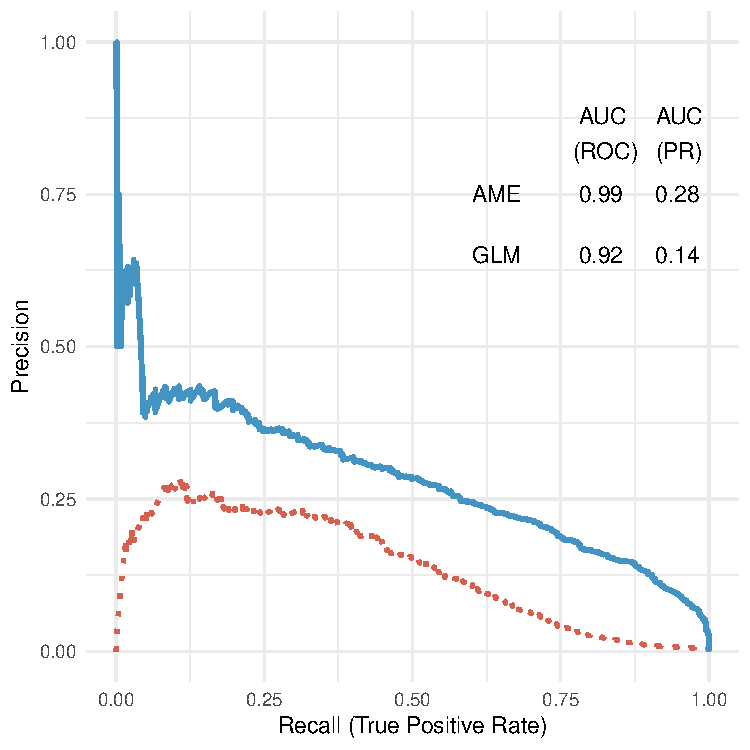
\includegraphics[width=.45\textwidth]{mcdonald_pr_outSample.pdf}}
% 	\caption{Assessments of out-of-sample predictive performance for McDonald (2004) using ROC curves and PR curves.}
% \end{figure}
\FloatBarrier

\clearpage
\subsubsection*{Weeks (2012)}

Coefficient plot and performance comparison.

% latex table generated in R 3.4.1 by xtable 1.8-2 package
% Sat Oct 21 23:26:08 2017
\begin{table}[ht]
\centering
\begingroup\scriptsize
\begin{tabular}{lccc}
 Variable & GLM (Logit) & GLM (Probit) & AME \\ 
  \hline
\hline
(Intercept) & $-3.784^{\ast\ast}$ & $-1.797^{\ast\ast}$ & $-2.409^{\ast\ast}$ \\ 
   & (0.423) & (0.159) & (0.132) \\ 
  Machine & $-0.459^{\ast\ast}$ & $-0.162^{\ast\ast}$ & -0.006 \\ 
   & (0.174) & (0.062) & (0.04) \\ 
  Junta & $0.515^{\ast\ast}$ & $0.194^{\ast\ast}$ & 0.034 \\ 
   & (0.169) & (0.062) & (0.046) \\ 
  Boss & $0.649^{\ast\ast}$ & $0.281^{\ast\ast}$ & -0.044 \\ 
   & (0.153) & (0.05) & (0.044) \\ 
  Strongman & $0.832^{\ast\ast}$ & $0.295^{\ast\ast}$ & 0.032 \\ 
   & (0.132) & (0.048) & (0.044) \\ 
  Other Type & 0.147 & 0.051 & -0.01 \\ 
   & (0.132) & (0.046) & (0.034) \\ 
  New/Unstable Regime & $-0.312^{\ast\ast}$ & $-0.123^{\ast\ast}$ & -0.043 \\ 
   & (0.092) & (0.033) & (0.031) \\ 
  Democracy Target & 0.185 & 0.052 & 0.024 \\ 
   & (0.115) & (0.04) & (0.026) \\ 
  Military Capabilities Initiator & $5.234^{\ast\ast}$ & $2.136^{\ast\ast}$ & 0.071 \\ 
   & (1.69) & (0.554) & (0.412) \\ 
  Military Capabilities Target  & $6.34^{\ast\ast}$ & $2.865^{\ast\ast}$ & $-0.969^{\ast\ast}$ \\ 
   & (1.675) & (0.573) & (0.48) \\ 
  Low Trade Dependence  & $-24.794^{\ast}$ & -8.197 & -4.733 \\ 
   & (12.866) & (5.582) & (3.017) \\ 
  Both Major Powers & $1.136^{\ast\ast}$ & $0.687^{\ast\ast}$ & $1.122^{\ast\ast}$ \\ 
   & (0.547) & (0.183) & (0.241) \\ 
  Minor/Major & $0.772^{\ast\ast}$ & $0.292^{\ast\ast}$ & $0.496^{\ast\ast}$ \\ 
   & (0.239) & (0.086) & (0.118) \\ 
  Major/Minor & $0.711^{\ast\ast}$ & $0.332^{\ast\ast}$ & $0.778^{\ast\ast}$ \\ 
   & (0.225) & (0.075) & (0.16) \\ 
  Contiguous & $2.172^{\ast\ast}$ & $0.738^{\ast\ast}$ & $0.705^{\ast\ast}$ \\ 
   & (0.32) & (0.125) & (0.06) \\ 
  Log Dist. Between Capitals & $-0.209^{\ast\ast}$ & $-0.095^{\ast\ast}$ & $-0.129^{\ast\ast}$ \\ 
   & (0.038) & (0.015) & (0.01) \\ 
  Alliance Similarity Dyad  & $-0.999^{\ast\ast}$ & $-0.386^{\ast\ast}$ & -0.073 \\ 
   & (0.144) & (0.05) & (0.065) \\ 
  Alliance Similarity With System Leader Initiator & 0.11 & 0.011 & 0.068 \\ 
   & (0.24) & (0.082) & (0.057) \\ 
  Alliance Similarity Leader Target & 0.203 & 0.032 & 0.08 \\ 
   & (0.244) & (0.081) & (0.056) \\ 
  Time Since Last Conflict & $-0.229^{\ast\ast}$ & $-0.089^{\ast\ast}$ & $-0.067^{\ast\ast}$ \\ 
   & (0.018) & (0.007) & (0.007) \\ 
  Spline1 & $-0.001^{\ast\ast}$ & $0.000^{\ast\ast}$ & $0.000^{\ast\ast}$ \\ 
   & (0.000) & (0.000) & (0.000) \\ 
  Spline2 & $0.000^{\ast\ast}$ & $0.000^{\ast\ast}$ & $0.000^{\ast\ast}$ \\ 
   & (0.000) & (0.000) & (0.000) \\ 
  Spline3 & 0.000 & 0.000 & 0.000 \\ 
   & (0.000) & (0.000) & (0.000) \\ 
   \hline
\hline
\end{tabular}
\endgroup
\caption{Parameter comparison for Weeks (2012). Standard errors in parentheses. $^{**}$ and $^{*}$ indicate significance at $p<0.05$ and $p<0.10$, respectively.} 
\label{tab:weeks_coef}
\end{table}

\FloatBarrier

% already show roc-pr in main text
% \begin{figure}
% 	\centering   
% 	\subfigure[AUC]{\label{fig:weeksroc}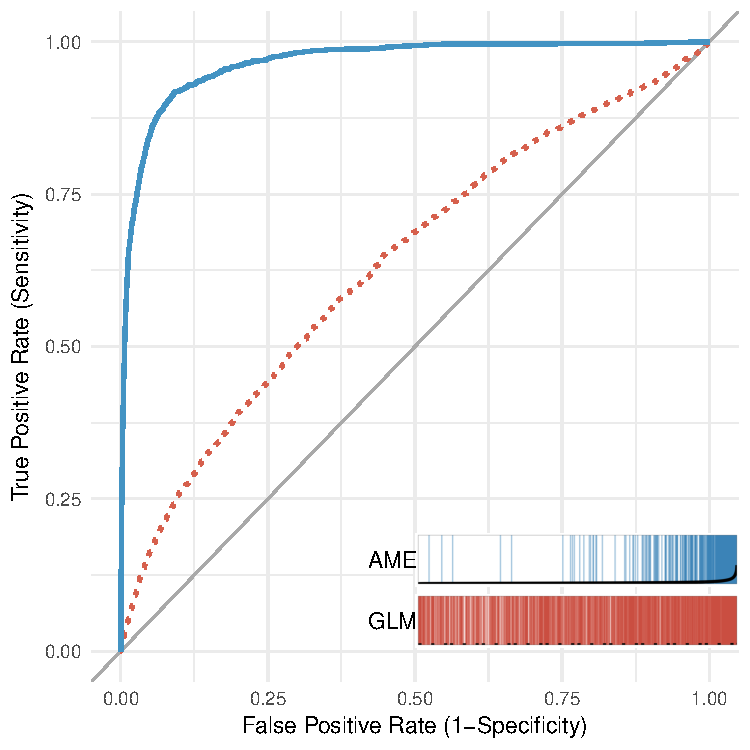
\includegraphics[width=.45\textwidth]{weeks_roc_outSample.pdf}}
% 	\subfigure[Precision and Recall]{\label{fig:weekspr}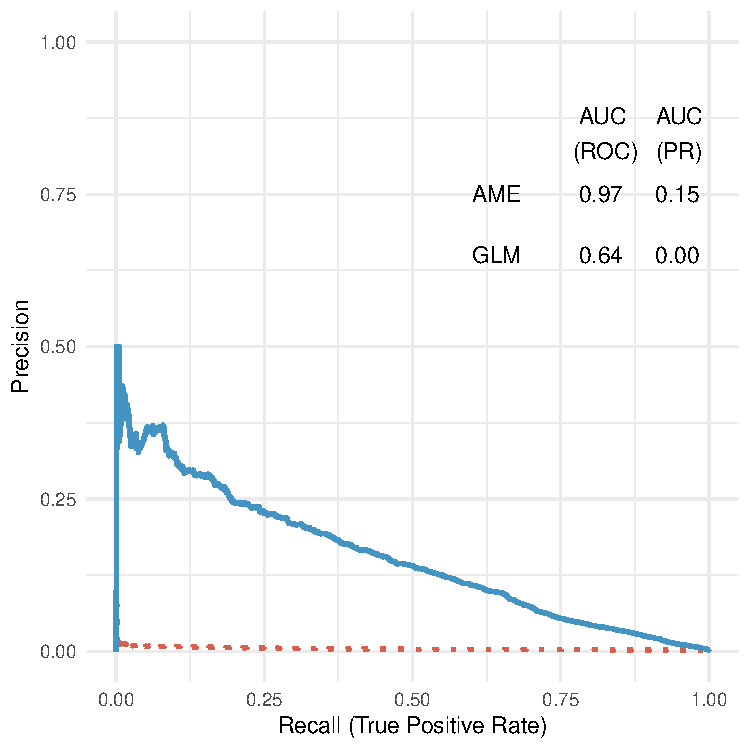
\includegraphics[width=.45\textwidth]{weeks_pr_outSample.pdf}}
% 	\caption{Assessments of out-of-sample predictive performance for Weeks (2012) using ROC curves and PR curves.}
% \end{figure}
% \FloatBarrier

\end{document}
